\chapter{Arhitektura i dizajn sustava}

\begin{packed_item}
			\item Struktura:
			\begin{packed_enum}
				\item Web poslužitelj
				\item \textit{Frontend} aplikacija
				\item \textit{Backend} aplikacija
				\item Baza podataka
			\end{packed_enum}
			\item REST stil web servisa
			\item ORM (objektno-relacijsko preslikavanje)
			\item Relacijska baza podataka
			\item \textit{Clean} arhitektura \textit{Backend}-a
		\end{packed_item}


		\textit{Web preglednik} je program pomoću kojeg korisnik može pristupati resursima na internetu. Ima ulogu klijenta koji traži resurse od dostupnih poslužitelja. U ovom slučaju, korisnik putem preglednika šalje zahtjev za dohvaćanje \textit{(Frontend) web aplikacije}, koja je implementirana kao \textit{SPA (engl. Single Page Application)} - statički servirana web stranica s dinamičkim kretanjem po sadržaju ovisno o putanji, bez obaveznog osvježavanja stranice.


		\textit{Frontend} (korisnička) aplikacija služi za komunikaciju s \textit{Backend} aplikacijom na poslužitelju, gdje se sva bitna poslovna logika aplikacije nalazi, a to omogućuje kroz korisničko sučelje.


		\textit{Backend} aplikacija prima korisničke zahtjeve i obrađuje ih, ovisno o zahtjevu korisnika pristupa bazi podataka te šalje potvrdne ili neuspješne odgovore prema korisničkoj aplikaciji, po potrebi i s dodatnim podacima u tijelu odgovora.

		\eject

		\section{Programski jezici, razvojni okviri, alati i biblioteke koda}

		\subsection{\textit{Backend} i baza podataka}
		U \textit{Backend} aplikaciji koristi se Java, Spring boot, JPA, Liquibase, PostgreSQL, XML, YAML, Gradle te JWT autentikacija/autorizacija.


		Spring boot je Java \textit{Framework} koji olakšava izradu web aplikacije kroz automatsku konfiguraciju ovisnih dijelova aplikacije unutar projekta te pruža razne implementacije tih dijelova koje apstrahiraju korištenje kroz intuitivna sučelja.


		\textit{Liquibase} se koristi za definiranje sheme baze podataka. JPA služi za preslikavanje entiteta iz \textit{PostgreSQL} baze podataka na klase u \textit{Backend} aplikaciji, a time se postiže lakše generiranje upita ovisno o pozivu metode na klasi entiteta.



		YAML je format datoteke korišten za konfiguracijske datoteke aplikacije, a XML za datoteke dnevnika promjena (engl. changelog). Za upravljanje bazom podataka koristi se DBeaver, a za realizaciju \textit{Backend} aplikacije Jetbrains IntelliJ Idea (Java). Za izgradnju cijele aplikacije koristi se Gradle, a za sigurnost se koristi \textit{JWT (engl. Json Web Token)} standard za generiranje tokena koji istovremeno služe za autorizaciju i autentikaciju korisnika.


		\subsection{\textit{Frontend}}
		Za \textit{Frontend} aplikaciju koristi se Typescript, React, TailwindCSS, Vite, React Query, Formik, HeadlessUI te Figma.


		React je \textit{Framework} koji olakšava izradu web stranica kroz razne implementacije za navigaciju, dohvaćanje te prikaz podataka. Za definiranje sadržaja stranice koristi označni kod sličan HTML-u, proširen mogućnostima Typescript-a. Za definiranje stila tj. izgleda stranice koristi se TailwindCSS.


		React Query koristi se za raspodjelu podataka u aplikaciji, za izradu formi koristi se biblioteka Formik, a za ponašanje kompleksnijih komponenti na stranici HeadlessUI. Vite je alat korišten za izgradnju cijele aplikacije.


		Dizajn ekrana aplikacije odrađen je pomoću alata Figma, a pisanje Typescripta u Visual Studio Code-u.







		\eject


		\section{Baza podataka}

		    Baza podataka korištena u projektu je PostgreSQL. 

			\subsection{Opis tablica}

				Trip - opisuje jedno objavljeno putovanje korisnika. U \textit{one to many} vezi s Location, \textit{many to one} sa User\_profile.

				\begin{longtblr}[
					label=none,
					entry=none
					]{
						width = \textwidth,
						colspec={|X[10,l]|X[6, l]|X[20, l]|},
						rowhead = 1,
					} %definicija širine tablice, širine stupaca, poravnanje i broja redaka naslova tablice
					\hline \multicolumn{3}{|c|}{\textbf{Trip}}	 \\ \hline[3pt]
					\SetCell{LightGreen}id & INT	&  	primarni ključ relacije Trip  	\\ \hline
					\SetCell{LightBlue}\textbf{user\_id}	& INT &  strani ključ od relacije User\_profile (User\_profile.user\_id) 	\\ \hline
					\SetCell{LightBlue}\textbf{location\_id} & INT &  strani ključ od relacije Location (Location.id)\\ \hline
					date\_visited & TIMESTAMP	&  	datum putovanja	\\ \hline
					upload\_timestamp & TIMESTAMP	&  	datum objave putovanja	\\ \hline
					transportation\_type & VARCHAR	&  	tip prijevoza	\\ \hline
					traffic\_rating & VARCHAR	&  	ocjena gužve na putovanju \\ \hline
					is\_solo & BOOLEAN	&  	samostalno ili putovanje u društvu	\\ \hline
					trip\_rating & VARCHAR	&  	ocjena putovanja	\\ \hline
					description & VARCHAR	&  	komentar na putovanje	\\ \hline
                        image & BYTEA & slika putovanja  \\ \hline
					%\SetCell{LightBlue} primjer	& VARCHAR &   	\\ \hline
				\end{longtblr}

				Trip\_like je veza \textit{many to many} između User\_profile i Trip.
				\begin{longtblr}[
					label=none,
					entry=none
					]{
						width = \textwidth,
						colspec={|X[10,l]|X[6, l]|X[20, l]|},
						rowhead = 1,
					}
					\hline \multicolumn{3}{|c|}{\textbf{Trip\_like}}	 \\ \hline[3pt]
					\SetCell{LightGreen}\textbf{user\_id} & INT	&  	primarni ključ relacije Trip\_like i strani ključ od relacije User\_profile (User\_profile.user\_id)	\\ \hline
					\SetCell{LightGreen}\textbf{trip\_id} & INT	&  	primarni ključ relacije Trip\_like i strani ključ od relacije Trip (Trip.id)	\\ \hline
					%\SetCell{LightBlue} primjer	& VARCHAR &   	\\ \hline
				\end{longtblr}

				Location - opisuje jednu lokaciju na karti. U \textit{one to many} vezi s Trip, \textit{many to one} vezi s City, \textit{one to many} sa Wishlist\_entry i \textit{many to one} s Account.
				\begin{longtblr}[
					label=none,
					entry=none
					]{
						width = \textwidth,
						colspec={|X[10,l]|X[6, l]|X[20, l]|},
						rowhead = 1,
					}
					%1:N trip
					%N:1 city
					%1:N wishlist entry
				    %N:N:N loc:userprf:badge
				    %N:1 account suggestioni
					\hline \multicolumn{3}{|c|}{\textbf{Location}}	 \\ \hline[3pt]
					\SetCell{LightGreen}id & INT	&  	  primarni ključ relacije Location  	\\ \hline
					name & VARCHAR	&  	ime lokacije	\\ \hline
					x\_coordinate	& INT &  x koordinata lokacije 	\\ \hline
					y\_coordinate & INT &  y koordinata lokacije \\ \hline
					type & VARCHAR	&  	tip lokacije (muzej, crkva...)	\\ \hline
					\SetCell{LightBlue}\textbf{city\_id} & INT &  strani ključ od relacije City (City.id)  \\ \hline
					is\_suggestion & BOOLEAN	&  	je li lokacija prijedlog regularnog korisnika	\\ \hline
					\SetCell{LightBlue}\textbf{suggested\_by\_user\_id}  & INT & strani ključ od relacije Account (Account.id)  \\ \hline
					%\SetCell{LightBlue} primjer	& VARCHAR &   	\\ \hline
				\end{longtblr}

				City - opisuje jedan grad. U \textit{one to many} vezi s Location i \textit{many to one} vezi s Country.
				\begin{longtblr}[
					label=none,
					entry=none
					]{
						width = \textwidth,
						colspec={|X[10,l]|X[6, l]|X[20, l]|},
						rowhead = 1,
					}
					%1:N loc
					%N:1 country
					\hline \multicolumn{3}{|c|}{\textbf{City}}	 \\ \hline[3pt]
					\SetCell{LightGreen}id & INT	&  	primarni ključ relacije City 	\\ \hline
					name & VARCHAR	&  ime grada		\\ \hline
					\SetCell{LightBlue}\textbf{country\_code} & INT &  strani ključ od relacije Country (Country.code)\\ \hline
					%\SetCell{LightBlue} primjer	& VARCHAR &   	\\ \hline
				\end{longtblr}

				Country - opisuje jednu državu. U \textit{one to many} vezi s City.
				\begin{longtblr}[
					label=none,
					entry=none
					]{
						width = \textwidth,
						colspec={|X[10,l]|X[6, l]|X[20, l]|},
						rowhead = 1,
					}
					%1:N city
					\hline \multicolumn{3}{|c|}{\textbf{Country}}	 \\ \hline[3pt]
					\SetCell{LightGreen}id & INT	&  	primarni ključ relacije Country 	\\ \hline
					name & VARCHAR	&  	ime države	\\ \hline
					%\SetCell{LightBlue} primjer	& VARCHAR &   	\\ \hline
				\end{longtblr}

				Wishlist\_entry - jedna želja na popisu želja. U \textit{many to one} vezi s Location, \textit{many to one} sa User\_profile te \textit{one to one} vezi s Badge.
				\begin{longtblr}[
					label=none,
					entry=none
					]{
						width = \textwidth,
						colspec={|X[10,l]|X[6, l]|X[20, l]|},
						rowhead = 1,
					}
					%N:1 lokacija
					%N:1 userpf
					%1:1 wishl badg
					\hline \multicolumn{3}{|c|}{\textbf{Wishlist\_entry}}	 \\ \hline[3pt]
					\SetCell{LightGreen}id & INT	&  	primarni ključ relacije Wishlist\_entry 	\\ \hline
					\SetCell{LightBlue}\textbf{user\_id} & INT &   strani ključ od relacije User\_profile (User\_profile.user\_id) \\ \hline
					\SetCell{LightBlue}\textbf{location\_id} & INT &   strani ključ od relacije Location (Location.id)\\ \hline
					visit\_before & TIMESTAMP &  deadline kada želja treba biti ispunjena  \\ \hline
					state & VARCHAR	&  	stanje	\\ \hline
					%\SetCell{LightBlue} primjer	& VARCHAR &   	\\ \hline
				\end{longtblr}

				Wishlist\_badge je veza između entiteta. \textit{One to one} veza Wishlist\_entry i Badge.
				\begin{longtblr}[
					label=none,
					entry=none
					]{
						width = \textwidth,
						colspec={|X[10,l]|X[6, l]|X[20, l]|},
						rowhead = 1,
					}
					%1:1 wishlist etny
					%0..1:1 badge
					\hline \multicolumn{3}{|c|}{\textbf{Wishlist\_badge}}	 \\ \hline[3pt]
					\SetCell{LightGreen}\textbf{id} & INT	&  	primarni ključ relacije Wishlist\_badge i strani ključ od relacije Badge 	\\ \hline
					\SetCell{LightBlue}\textbf{wishlist\_entry\_id} & INT &   strani ključ od relacije Wishlist\_entry (Wishlist\_entry.id) \\ \hline
					%\SetCell{LightBlue} primjer	& VARCHAR &   	\\ \hline
				\end{longtblr}

				Won\_badge je veza \textit{many to many to many} Location, User\_profile, Badge.
				\begin{longtblr}[
					label=none,
					entry=none
					]{
						width = \textwidth,
						colspec={|X[10,l]|X[6, l]|X[20, l]|},
						rowhead = 1,
					}

					\hline \multicolumn{3}{|c|}{\textbf{Won\_badge}}	 \\ \hline[3pt]
					\SetCell{LightGreen}\textbf{user\_id} & INT	&  	primarni ključ relacije Won\_badge i strani ključ od relacije User\_profile (User\_profile.user\_id)	\\ \hline
					\SetCell{LightGreen}\textbf{badge\_id} & INT & primarni i strani ključ od relacije Badge (Badge.id) \\ \hline
					\SetCell{LightGreen}\textbf{last\_location\_id} & INT & primarni i strani ključ od relacije Location (Location.id) \\ \hline
					won\_timestamp & TIMESTAMP & datum osvajanja bedža   \\ \hline
					%\SetCell{LightBlue} primjer	& VARCHAR &   	\\ \hline
				\end{longtblr}

				Badge - opisuje jedan bedž. U \textit{one to one} vezi s City\_badge i \textit{one to one} vezi s Country\_badge.
				\begin{longtblr}[
					label=none,
					entry=none
					]{
						width = \textwidth,
						colspec={|X[10,l]|X[6, l]|X[20, l]|},
						rowhead = 1,
					}
					%1:0..1 wish bacge
					%1:0..1 ctry bdg
					%1:0..1 city bdg
					%N:N:N loc:userprf:badge
					\hline \multicolumn{3}{|c|}{\textbf{Badge}}	 \\ \hline[3pt]
					\SetCell{LightGreen}id & INT	&  	primarni ključ relacije Badge 	\\ \hline
					name & VARCHAR	&  	ime bedža	\\ \hline
					image & INT &   slika bedža  \\ \hline
					type & VARCHAR	&  	tip bedža	\\ \hline
                        image & BYTEA & slika bedža  \\ \hline
					%\SetCell{LightBlue} primjer	& VARCHAR &   	\\ \hline
				\end{longtblr}

				City\_badge - opisuje pravila za gradove. U \textit{one to one} vezi s Badge i \textit{one to many} vezi s City\_badge\_requirement.
				\begin{longtblr}[
					label=none,
					entry=none
					]{
						width = \textwidth,
						colspec={|X[10,l]|X[6, l]|X[20, l]|},
						rowhead = 1,
					}
					%0..1:1 badge
					%1:N city badge req
					\hline \multicolumn{3}{|c|}{\textbf{City\_badge}}	 \\ \hline[3pt]
					\SetCell{LightGreen}\textbf{id} & INT	&  primarni relacije City i strani ključ od relacije Badge (Badge.id)	\\ \hline
					required\_locations & INT &  broj koliko minimalno lokacija unutar grada treba posjetiti  \\ \hline
					%\SetCell{LightBlue} primjer	& VARCHAR &   	\\ \hline
				\end{longtblr}

				City\_badge\_requirement - opisuje pravila lokacija unutar grada. U \textit{many to one} vezi s City\_badge.
				\begin{longtblr}[
					label=none,
					entry=none
					]{
						width = \textwidth,
						colspec={|X[10,l]|X[6, l]|X[20, l]|},
						rowhead = 1,
					}
					%N:1 city bdg
					\hline \multicolumn{3}{|c|}{\textbf{City\_badge\_requirement}}	 \\ \hline[3pt]
					\SetCell{LightGreen}id & INT	&  primarni	ključ relacije City\_badge\_requirement 	\\ \hline
					\SetCell{LightBlue}\textbf{badge\_id} & INT &   strani ključ od relacije City\_badge (City\_badge.id)\\ \hline
					required\_locations & INT &  broj koliko minimalno lokacija tipa \textbf{location\_type} unutar grada treba posjetiti   \\ \hline
					location\_type & VARCHAR	&  	tip lokacije	\\ \hline
					%\SetCell{LightBlue} primjer	& VARCHAR &   	\\ \hline
				\end{longtblr}

				Country\_badge - opisuje pravila za države. U \textit{one to one} vezi s Badge.
				\begin{longtblr}[
					label=none,
					entry=none
					]{
						width = \textwidth,
						colspec={|X[10,l]|X[6, l]|X[20, l]|},
						rowhead = 1,
					}
					%0..1:1 badge
					\hline \multicolumn{3}{|c|}{\textbf{Country\_badge}}	 \\ \hline[3pt]
					\SetCell{LightGreen}\textbf{id} & INT	&  primarni ključ relacije Country\_badge i strani ključ relacije od relacije Badge (Badge.id)	\\ \hline
					visit\_capital\_city & BOOLEAN &  je li potrebno posjetiti glavni grad  \\ \hline
					required\_number & INT &  ako je potrebno posjetiti glavni grad, broj \textbf{type} koje je potrebno posjetiti izvan glavnog grad. ako nije potrebno posjetiti glavni grad, broj \textbf{type} koje je potrebno posjetiti unutar države\\ \hline
					type & VARCHAR	&  enumeracija: grad, lokacija	\\ \hline
					%\SetCell{LightBlue} primjer	& VARCHAR &   	\\ \hline
				\end{longtblr}

				Account - opisuje jedan korisnički račun. U \textit{one to one} vezi sa User\_profile i \textit{one to many} vezi s Location.
				\begin{longtblr}[
					label=none,
					entry=none
					]{
						width = \textwidth,
						colspec={|X[10,l]|X[6, l]|X[20, l]|},
						rowhead = 1,
					}
					%1:1 usr pf
					%n:n role
					%1:n location
					\hline \multicolumn{3}{|c|}{\textbf{Account}}	 \\ \hline[3pt]
					\SetCell{LightGreen}id & INT	&  	primarni ključ relacije Account 	\\ \hline
					name & VARCHAR	&  	ime korisnika	\\ \hline
					surname & VARCHAR	&  	prezime korisnika	\\ \hline
					username & VARCHAR	&  	korisničko ime korisnika	\\ \hline
					email & VARCHAR	&  	email korisnika	\\ \hline
				    password & VARCHAR	&  lozinka korisnika		\\ \hline
					is\_active & BOOLEAN &  je li korisnikov račun aktivan  \\ \hline
					%\SetCell{LightBlue} primjer	& VARCHAR &   	\\ \hline
				\end{longtblr}

				User\_profile - opisuje jedan korisnički profil. U \textit{one to one} vezi s Account, \textit{one to many} vezi sa Trip i \textit{one to many} vezi sa Wishlist\_entry.
				\begin{longtblr}[
					label=none,
					entry=none
					]{
						width = \textwidth,
						colspec={|X[10,l]|X[6, l]|X[20, l]|},
						rowhead = 1,
					}
					%n:n user pf firend
					%n:n trip (trip_like)
					%1:1 acc
					%1:n trip
					%:N:N loc:userprf:badge
					%1:n wishlist entry
					\hline \multicolumn{3}{|c|}{\textbf{User\_profile}}	 \\ \hline[3pt]
					\SetCell{LightGreen}\textbf{user\_id} & INT	& primarni ključ relacije User\_profile i strani ključ relacije od relacije Account (Account.id) 	\\ \hline
					is\_public & BOOLEAN &  je li profil javan, prikazuju li se putovanja  \\ \hline
					profile\_image & BYTEA & slika korisničkog profila  \\ \hline
					%\SetCell{LightBlue} primjer	& VARCHAR &   	\\ \hline
				\end{longtblr}

				Friend je veza \textit{many to many} između User\_profile i User\_profile.
				\begin{longtblr}[
					label=none,
					entry=none
					]{
						width = \textwidth,
						colspec={|X[10,l]|X[6, l]|X[20, l]|},
						rowhead = 1,
					}
					\hline \multicolumn{3}{|c|}{\textbf{Friend}}	 \\ \hline[3pt]
					\SetCell{LightGreen}\textbf{from\_user\_id} & INT	&  primarni ključ relacije Friend i strani ključ od relacije User\_profile (User\_profile.user\_id) \\ \hline
					\SetCell{LightGreen}\textbf{to\_user\_id} & INT	&  	primarni ključ relacije Friend i strani ključ od relacije User\_profile (User\_profile.user\_id)\\ \hline
					is\_trip\_friend & BOOLEAN &  je li prijatelj označeno kao prijatelj s putovanja  \\ \hline
					%\SetCell{LightBlue} primjer	& VARCHAR &   	\\ \hline
				\end{longtblr}

				User\_role je veza \textit{many to many} između Account i Role.
				\begin{longtblr}[
					label=none,
					entry=none
					]{
						width = \textwidth,
						colspec={|X[10,l]|X[6, l]|X[20, l]|},
						rowhead = 1,
					}
					\hline \multicolumn{3}{|c|}{\textbf{User\_role}}	 \\ \hline[3pt]
					\SetCell{LightGreen}\textbf{user\_id} & INT	&  	primarni ključ relacije User\_role i strani ključ od relacije Account \\ \hline
					\SetCell{LightGreen}\textbf{role\_id} & INT	&  	primarni ključ relacije User\_role i strani ključ od relacije Role \\ \hline
					%\SetCell{LightBlue} primjer	& VARCHAR &   	\\ \hline
				\end{longtblr}

				Role - opisuje jednu korisničku ulogu.
				\begin{longtblr}[
					label=none,
					entry=none
					]{
						width = \textwidth,
						colspec={|X[10,l]|X[6, l]|X[20, l]|},
						rowhead = 1,
					}
					%n:n account (user:_role)
					\hline \multicolumn{3}{|c|}{\textbf{Role}}	 \\ \hline[3pt]
					\SetCell{LightGreen}id & INT	&  primarni	ključ relacije Role \\ \hline
					name & VARCHAR & ime uloge\\ \hline
					%\SetCell{LightBlue} primjer	& VARCHAR &   	\\ \hline
				\end{longtblr}







			\subsection{Dijagram baze podataka}
				\begin{figure}[H]
        			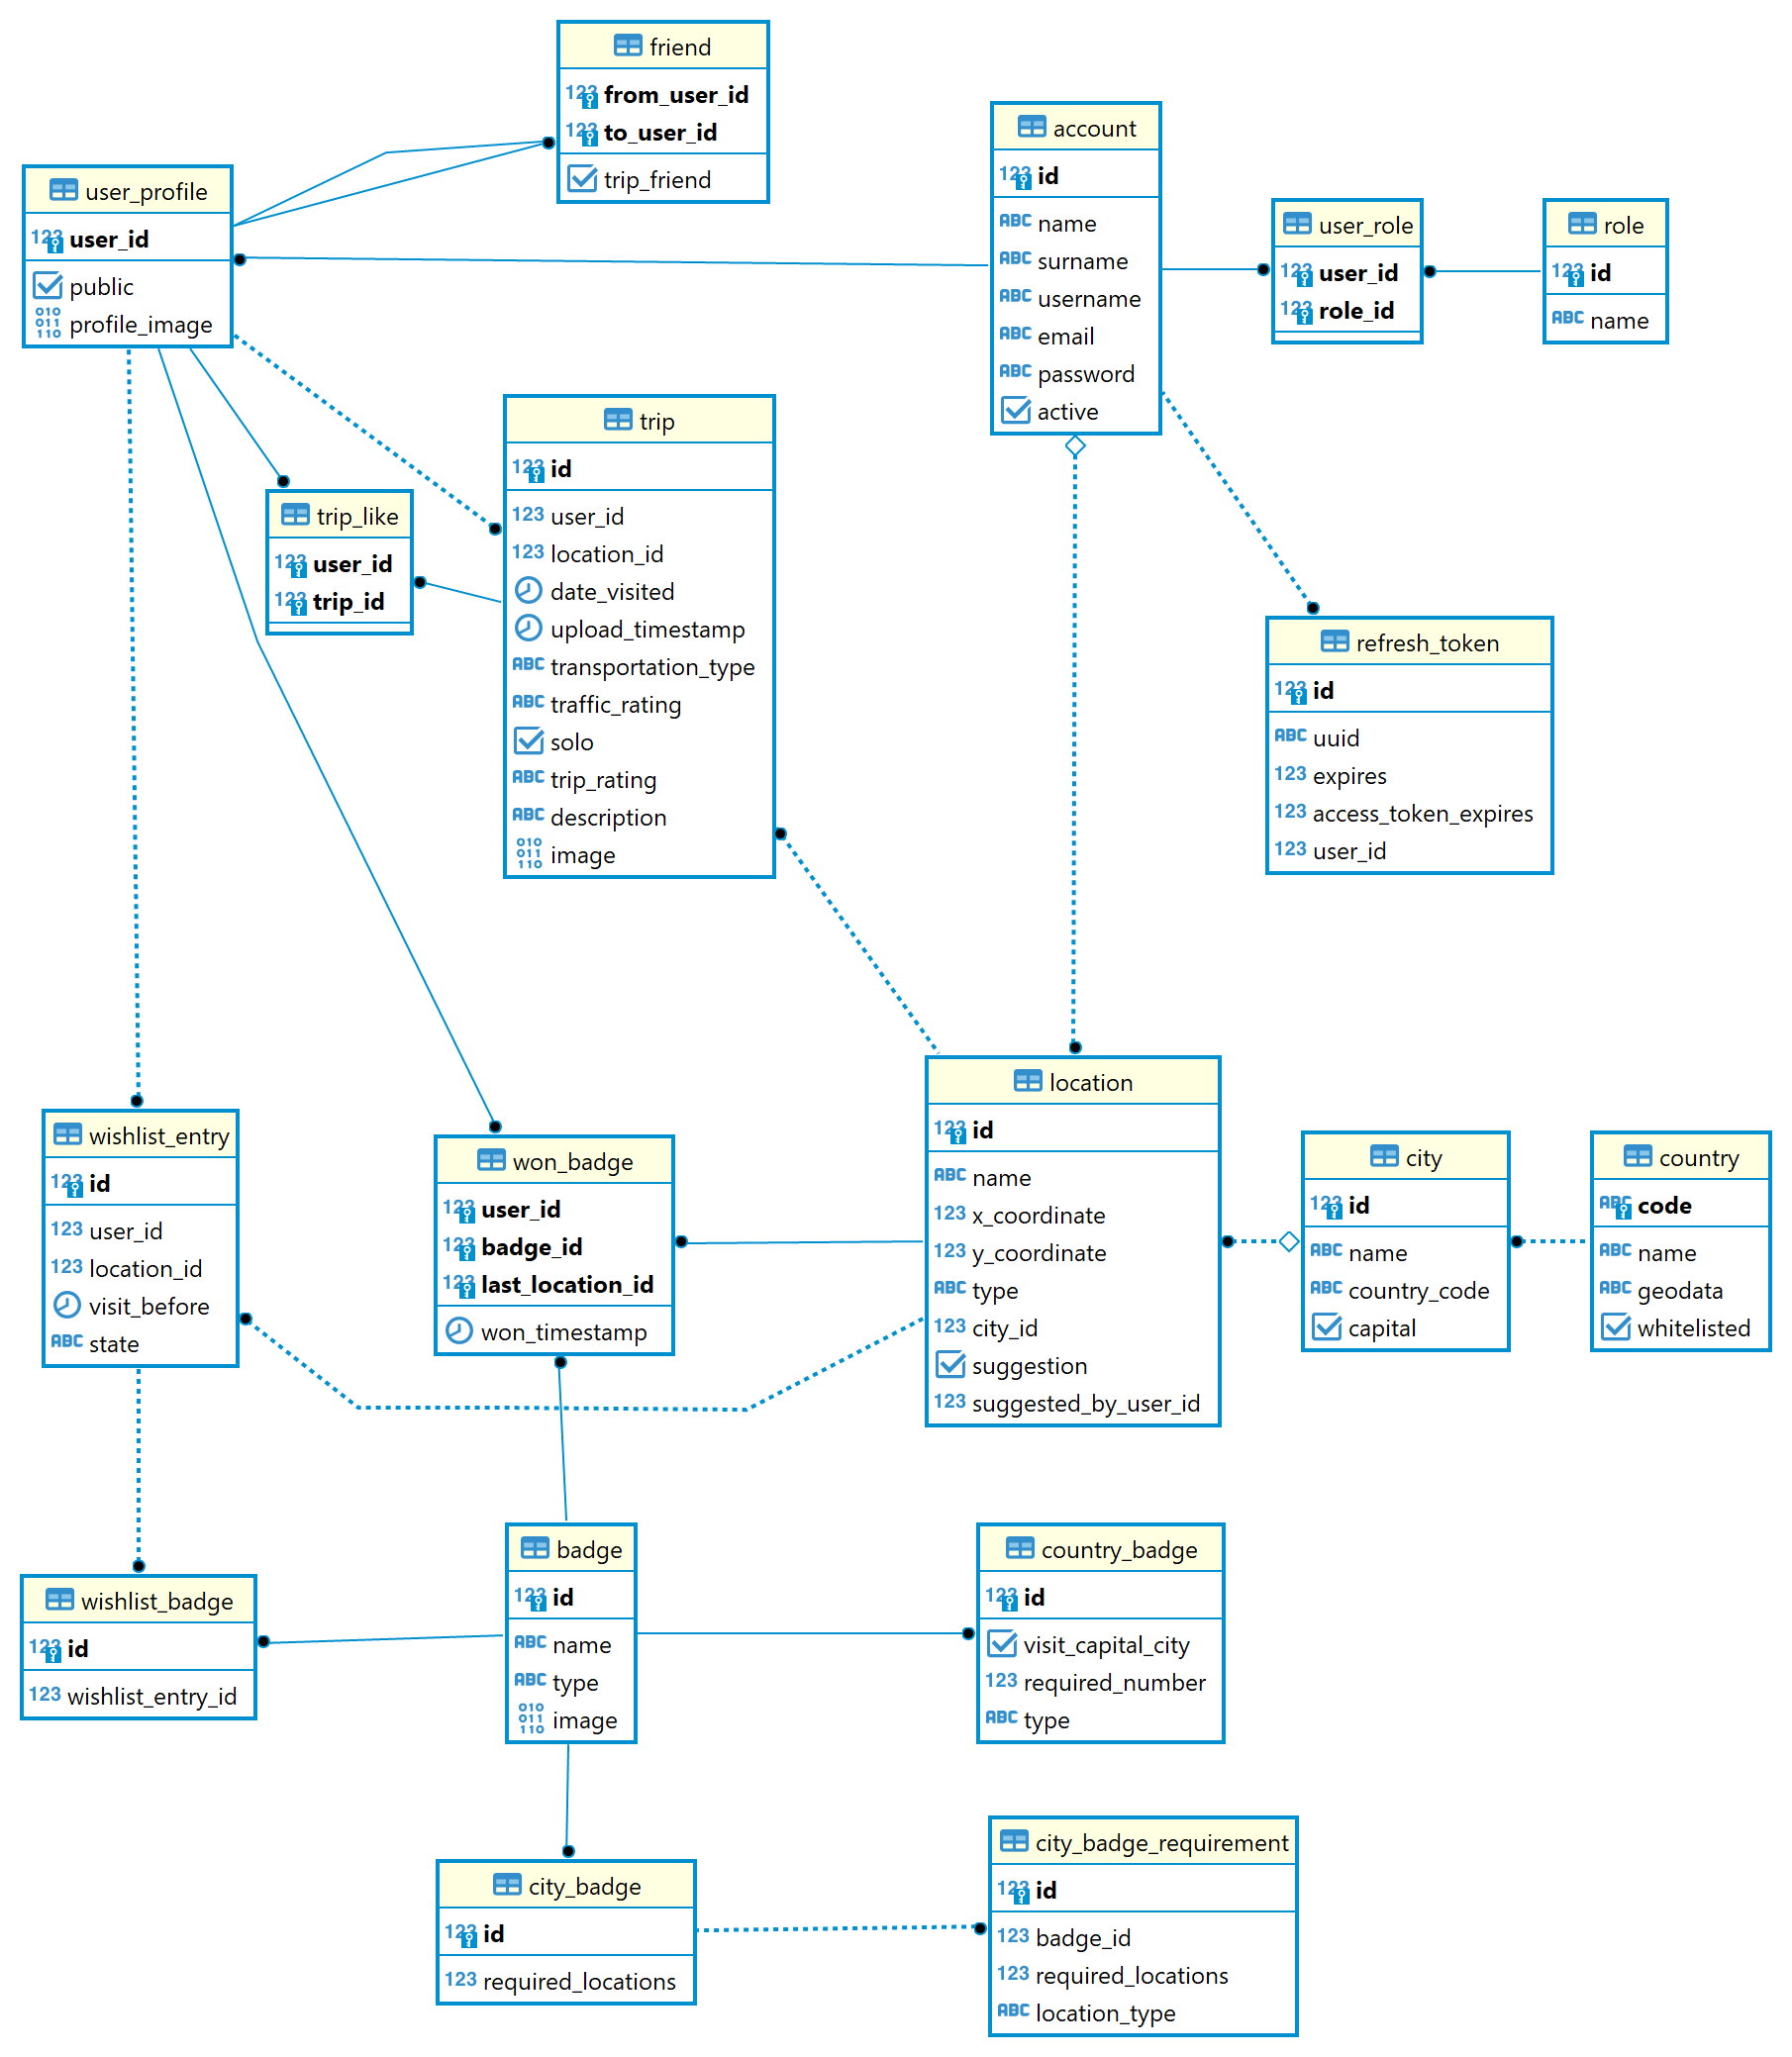
\includegraphics[scale=0.2]{slike/dijagram_baze.png} %veličina slike u odnosu na originalnu datoteku i pozicija slike
        			\centering
        			\caption{Dijagram baze podataka}

        		\end{figure}


		\section{Dijagram razreda}

                \begin{figure}[H]
        			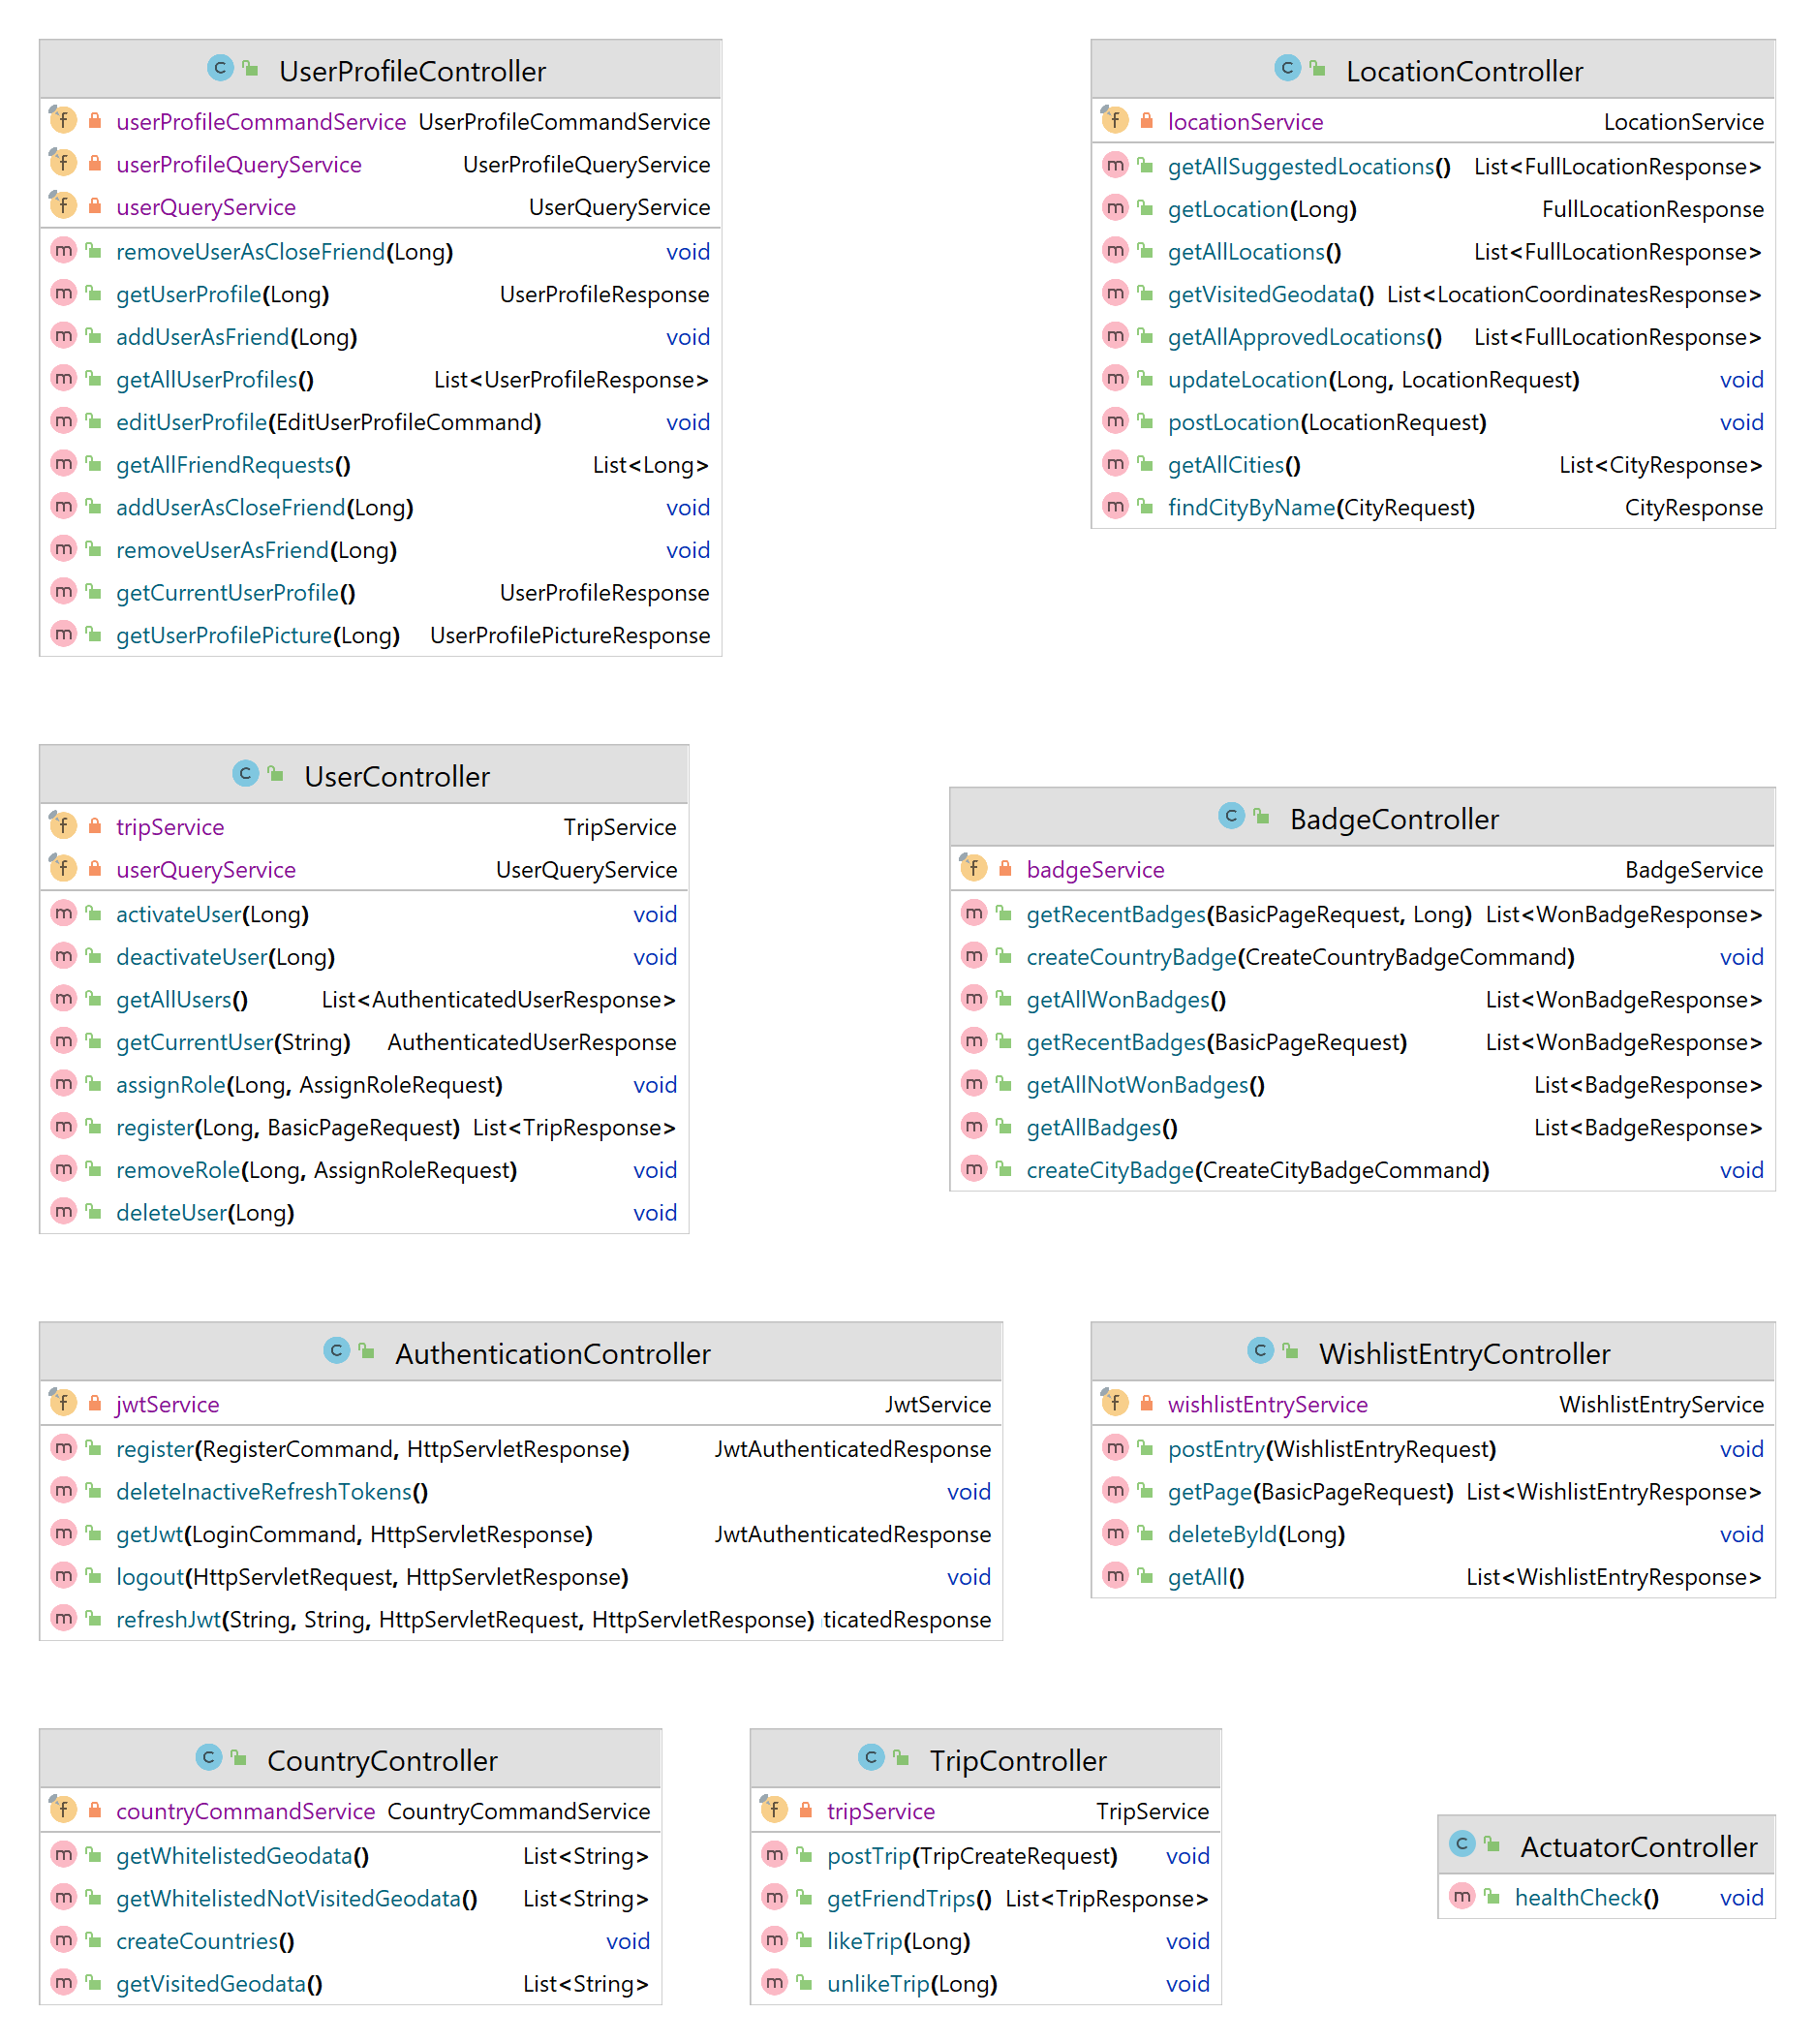
\includegraphics[scale=0.2]{slike/class/class_controller.png} %veličina slike u odnosu na originalnu datoteku i pozicija slike
        		\centering
        		\caption{Dijagram razreda - \textit{Controller}}

        	\end{figure}

                \begin{figure}[H]
        			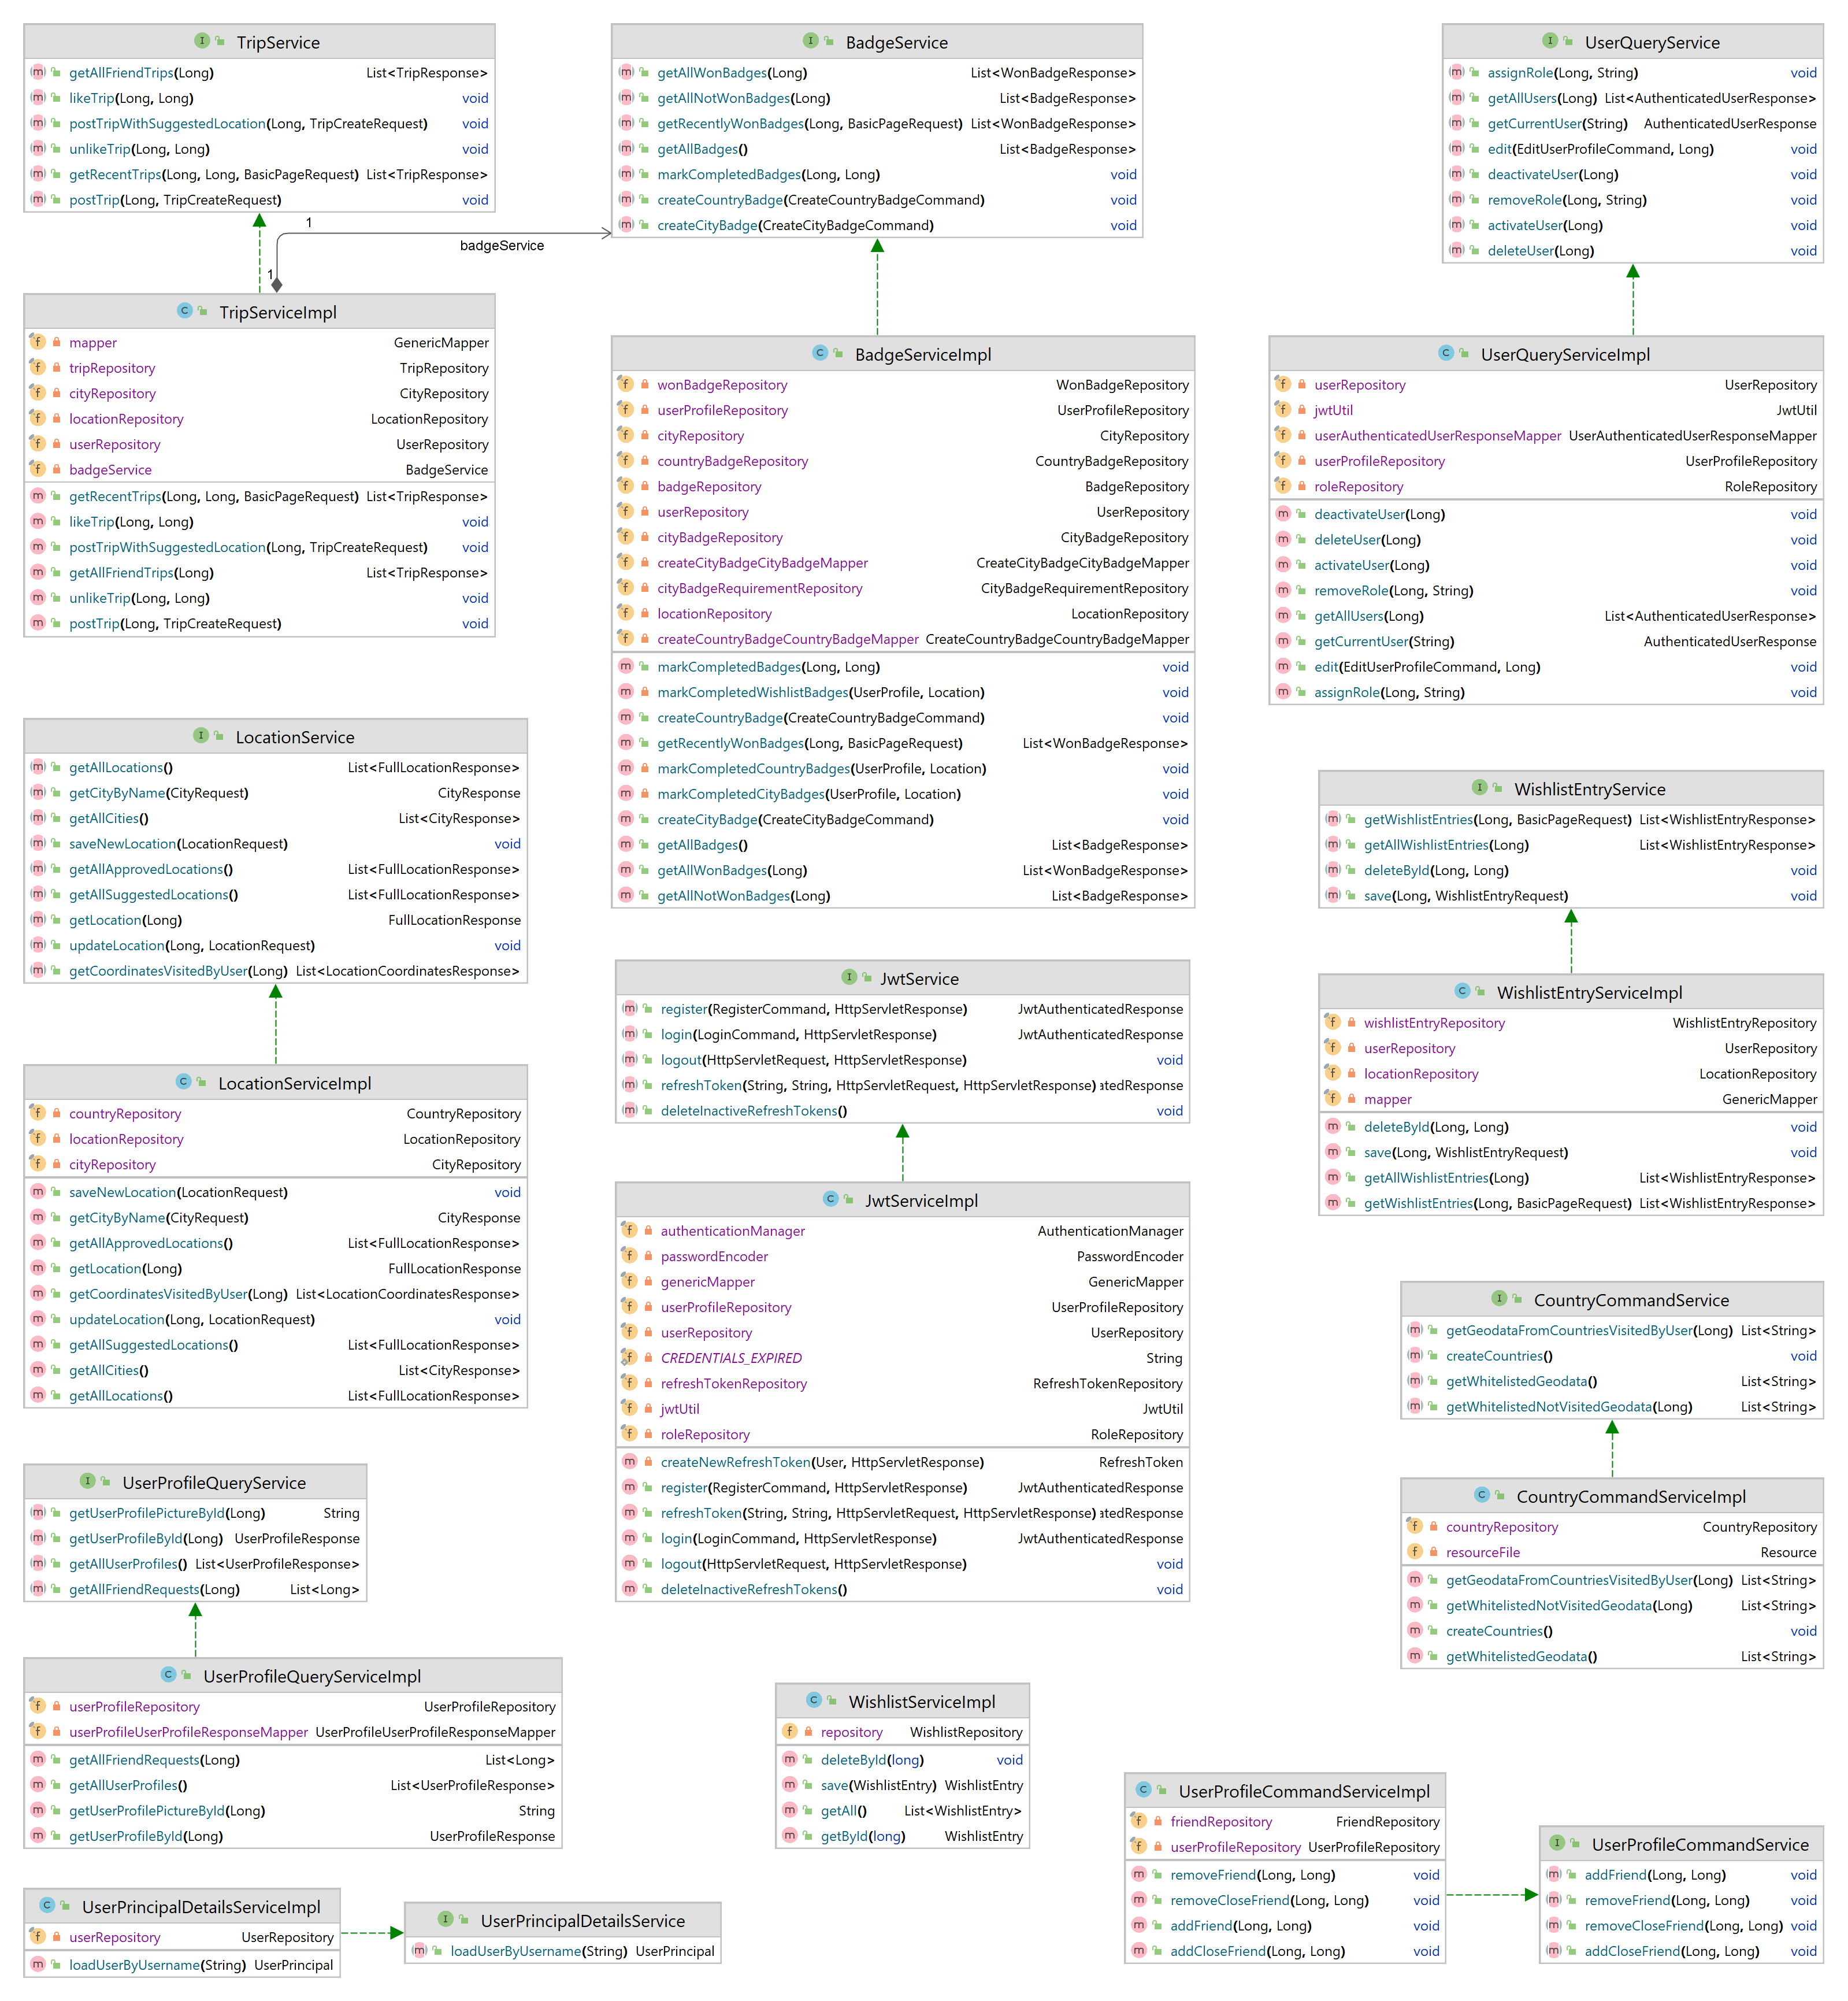
\includegraphics[scale=0.12]{slike/class/class_service.png} %veličina slike u odnosu na originalnu datoteku i pozicija slike
        		\centering
        		\caption{Dijagram razreda - \textit{Service}}
        	\end{figure}

                 \begin{figure}[H]
        			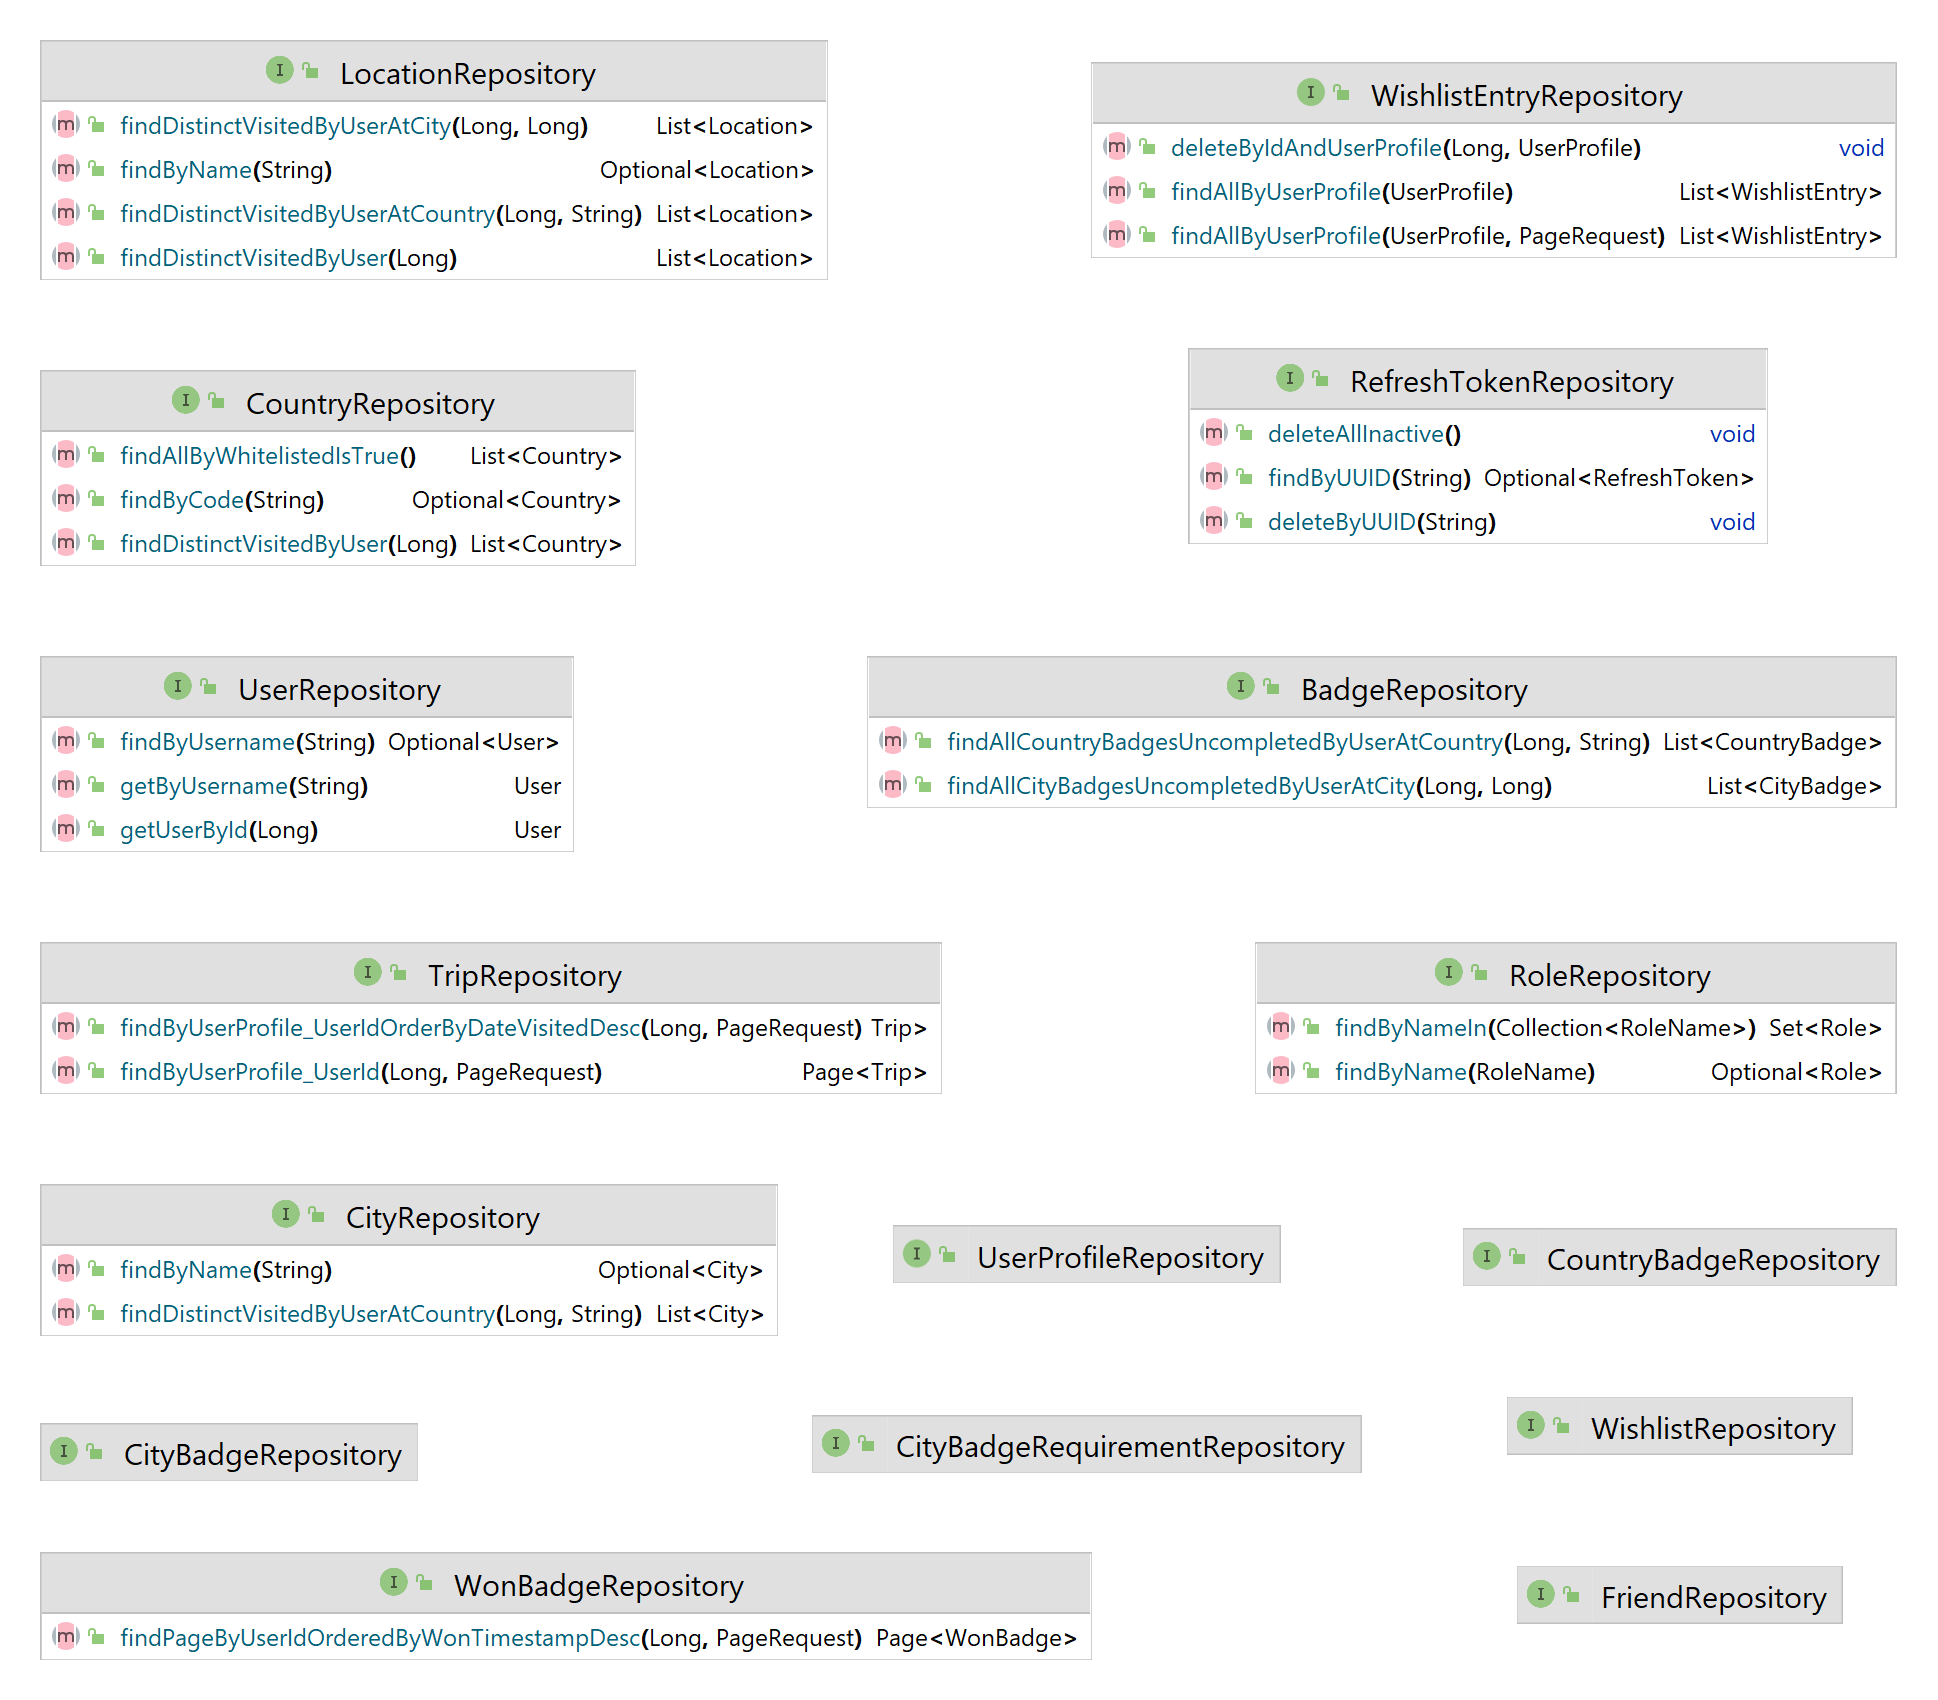
\includegraphics[scale=0.2]{slike/class/class_respository.png} %veličina slike u odnosu na originalnu datoteku i pozicija slike
        		\centering
        		\caption{Dijagram razreda - \textit{Repository}}

        	\end{figure}
                \eject
        
                \begin{figure}[H]
        			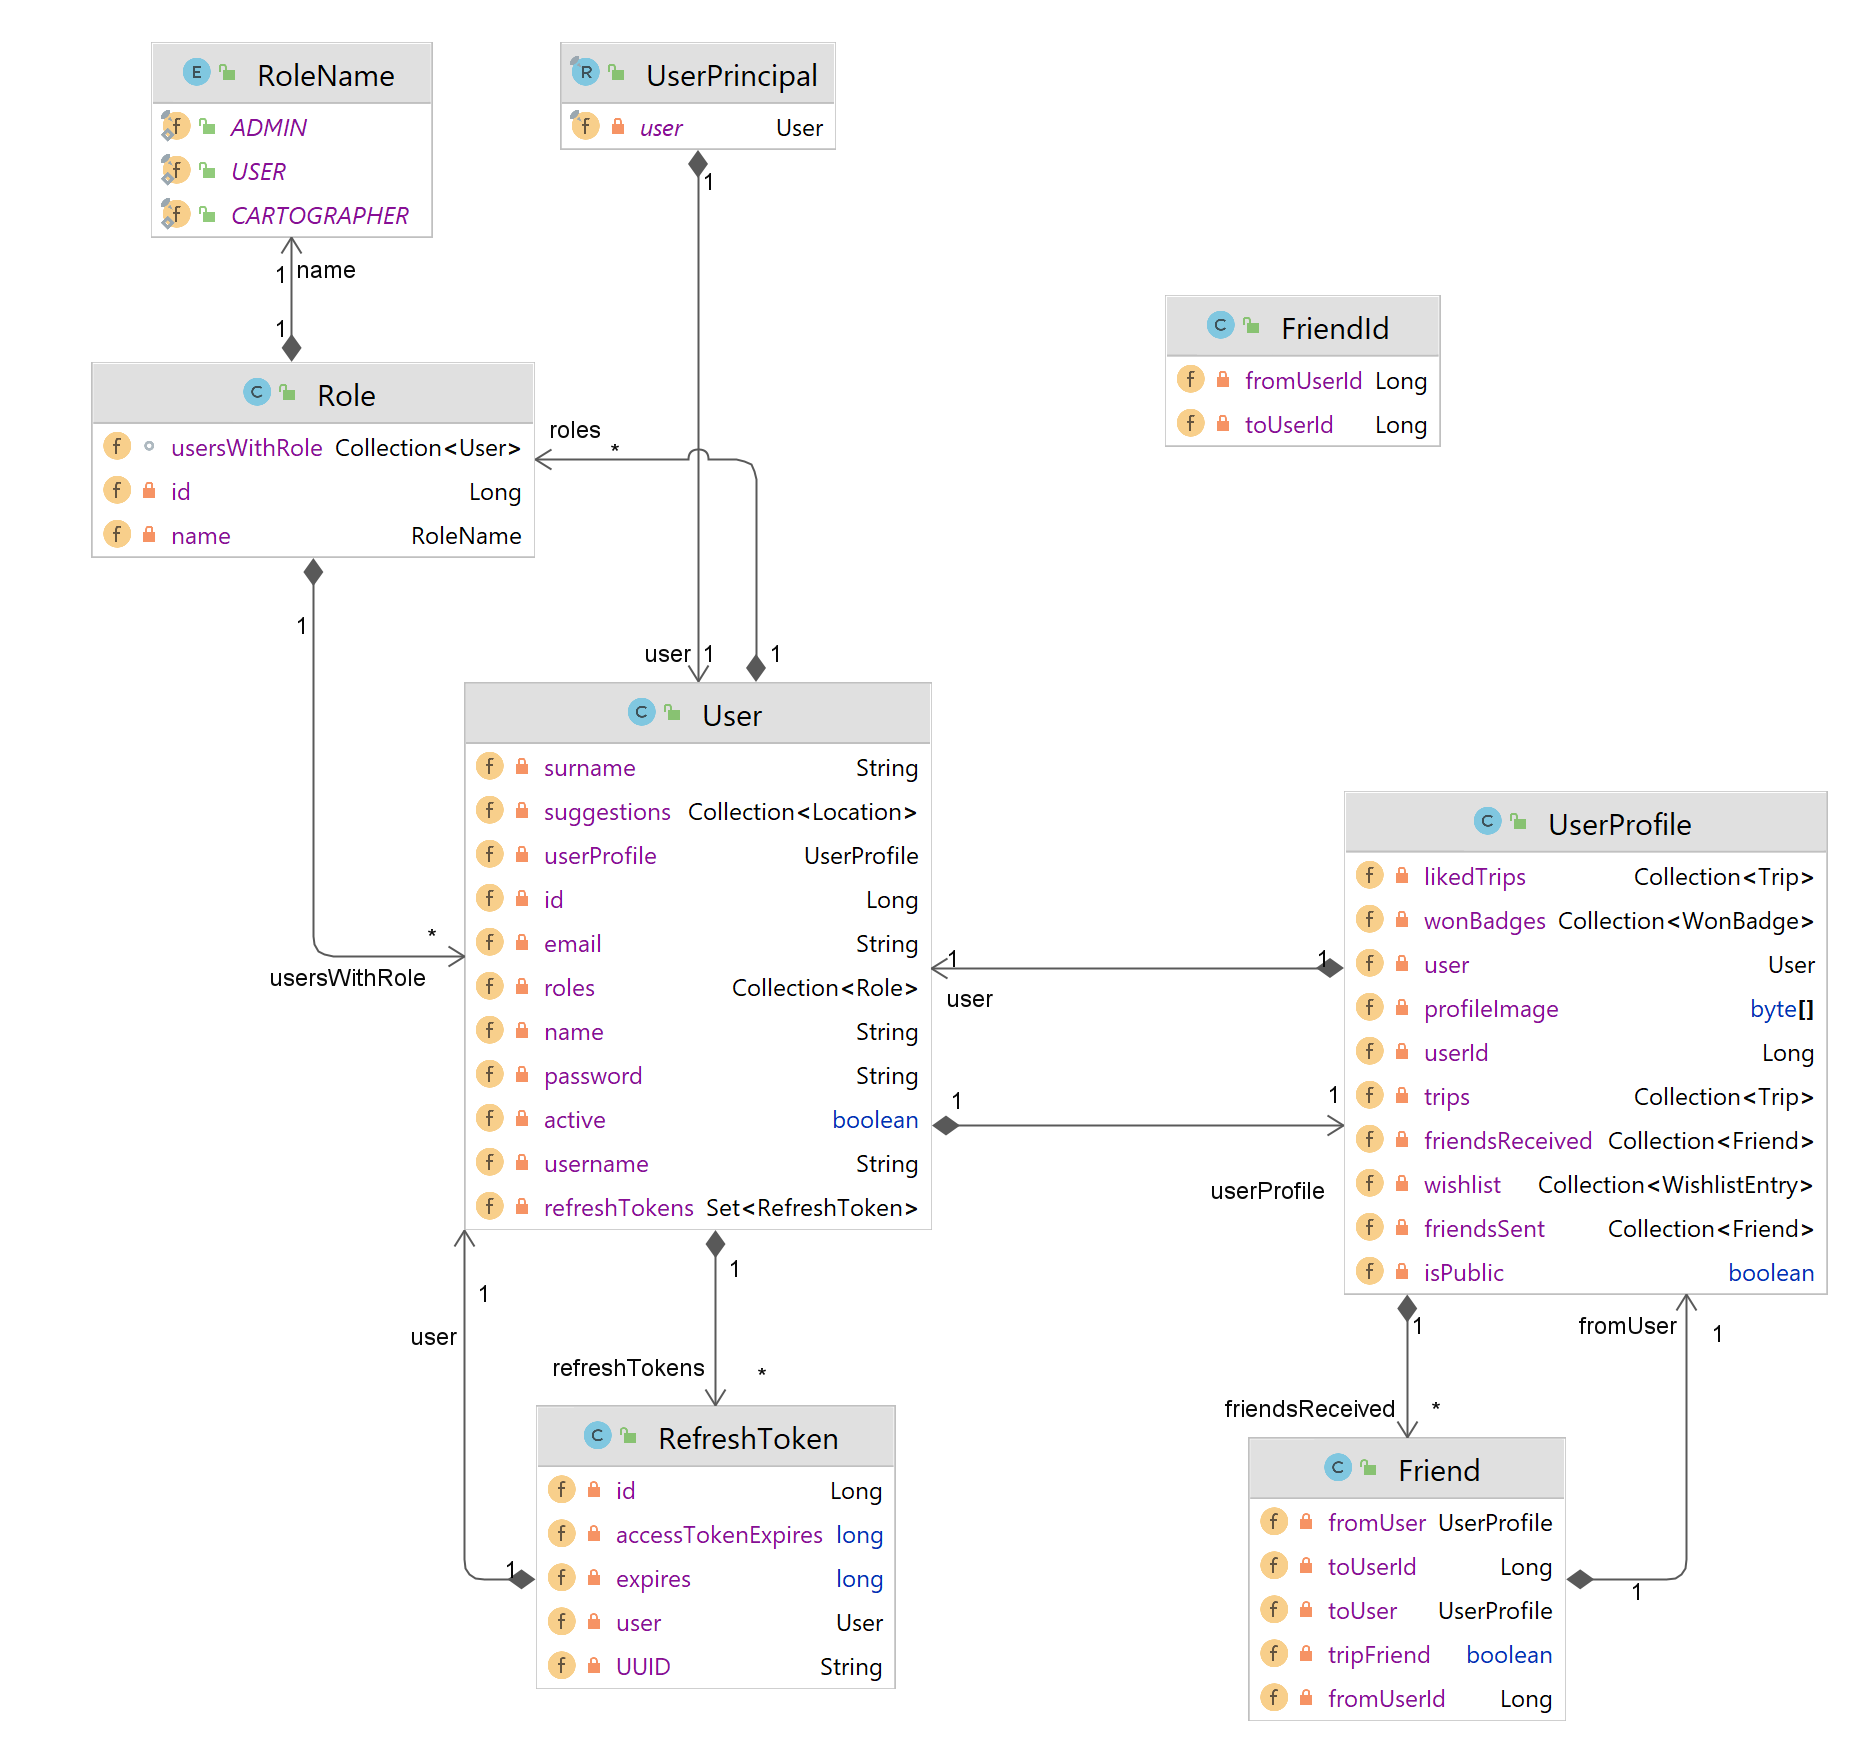
\includegraphics[scale=0.2]{slike/class/class_model_user.png}
        		\centering
        		\caption{Dijagram razreda - modeli korisnika}
        	\end{figure}
         
                \begin{figure}[H]
        			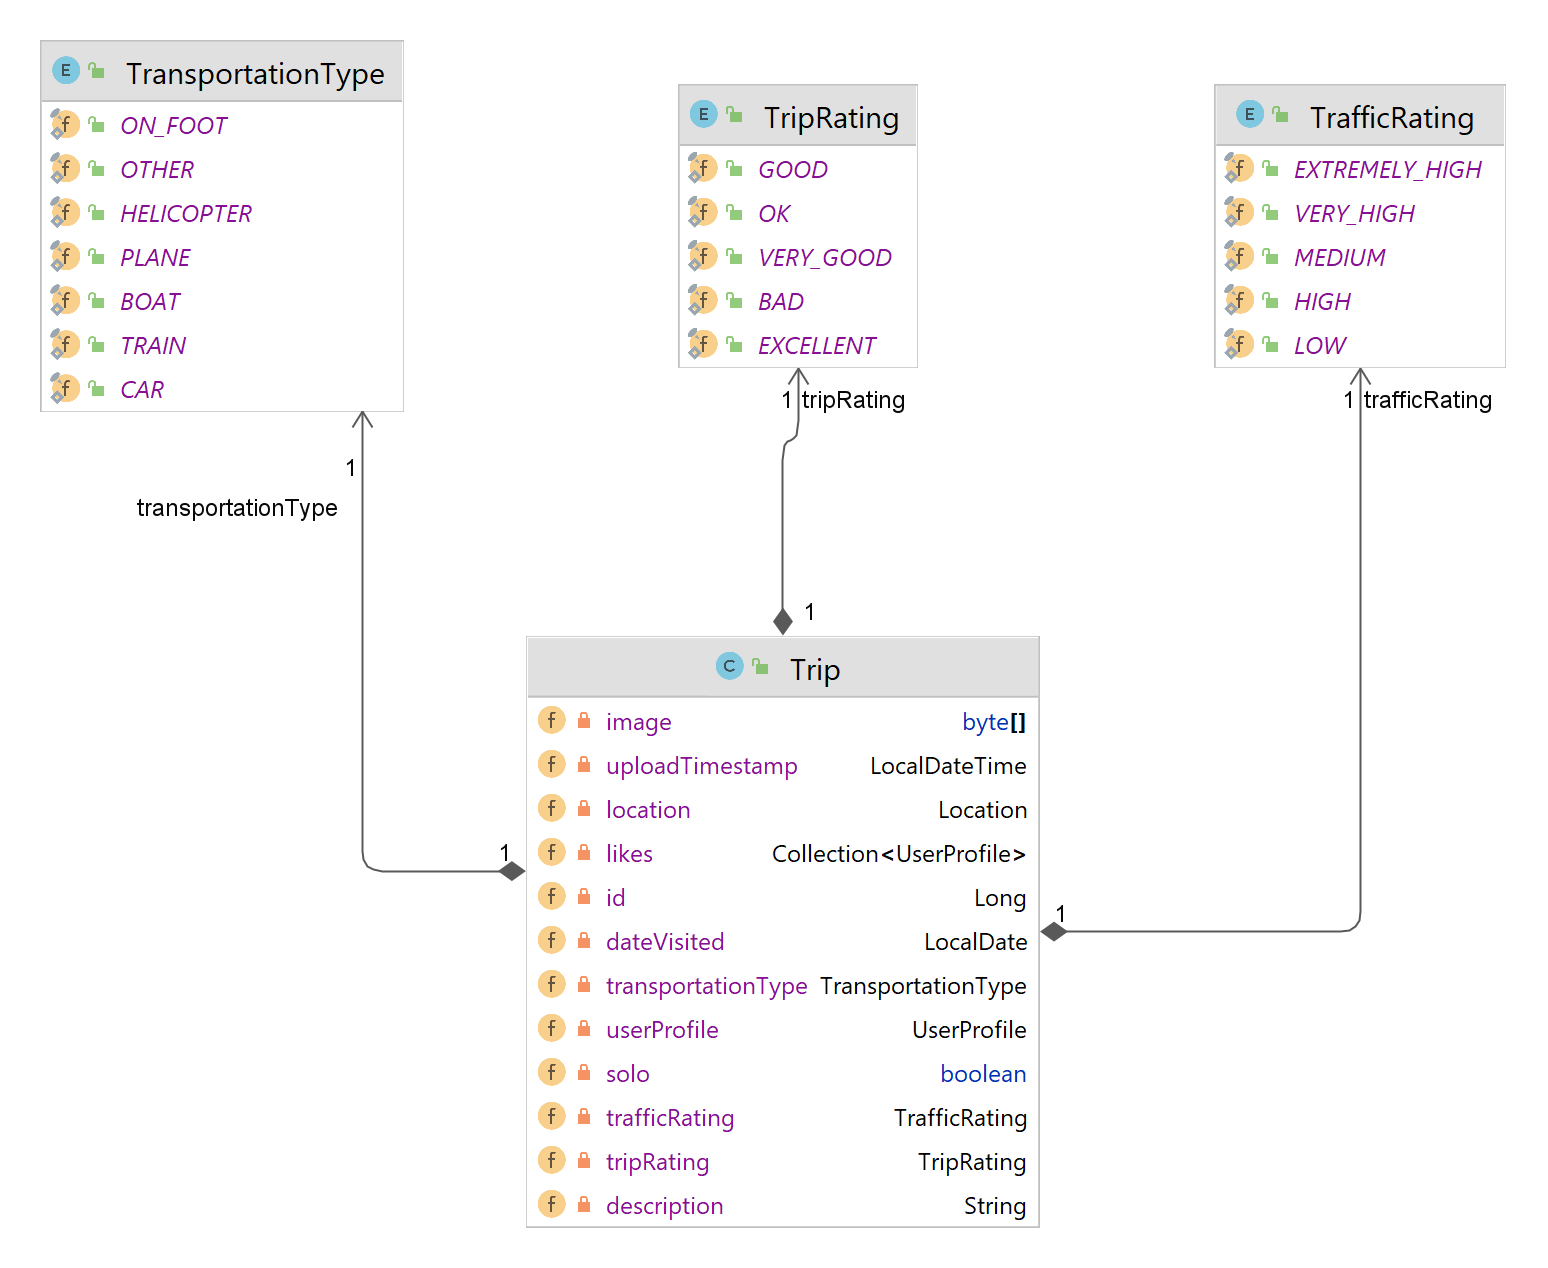
\includegraphics[scale=0.2]{slike/class/class_model_trip.png}
        		\centering
        		\caption{Dijagram razreda - modeli putovanja}
        	\end{figure}

                \begin{figure}[H]
        			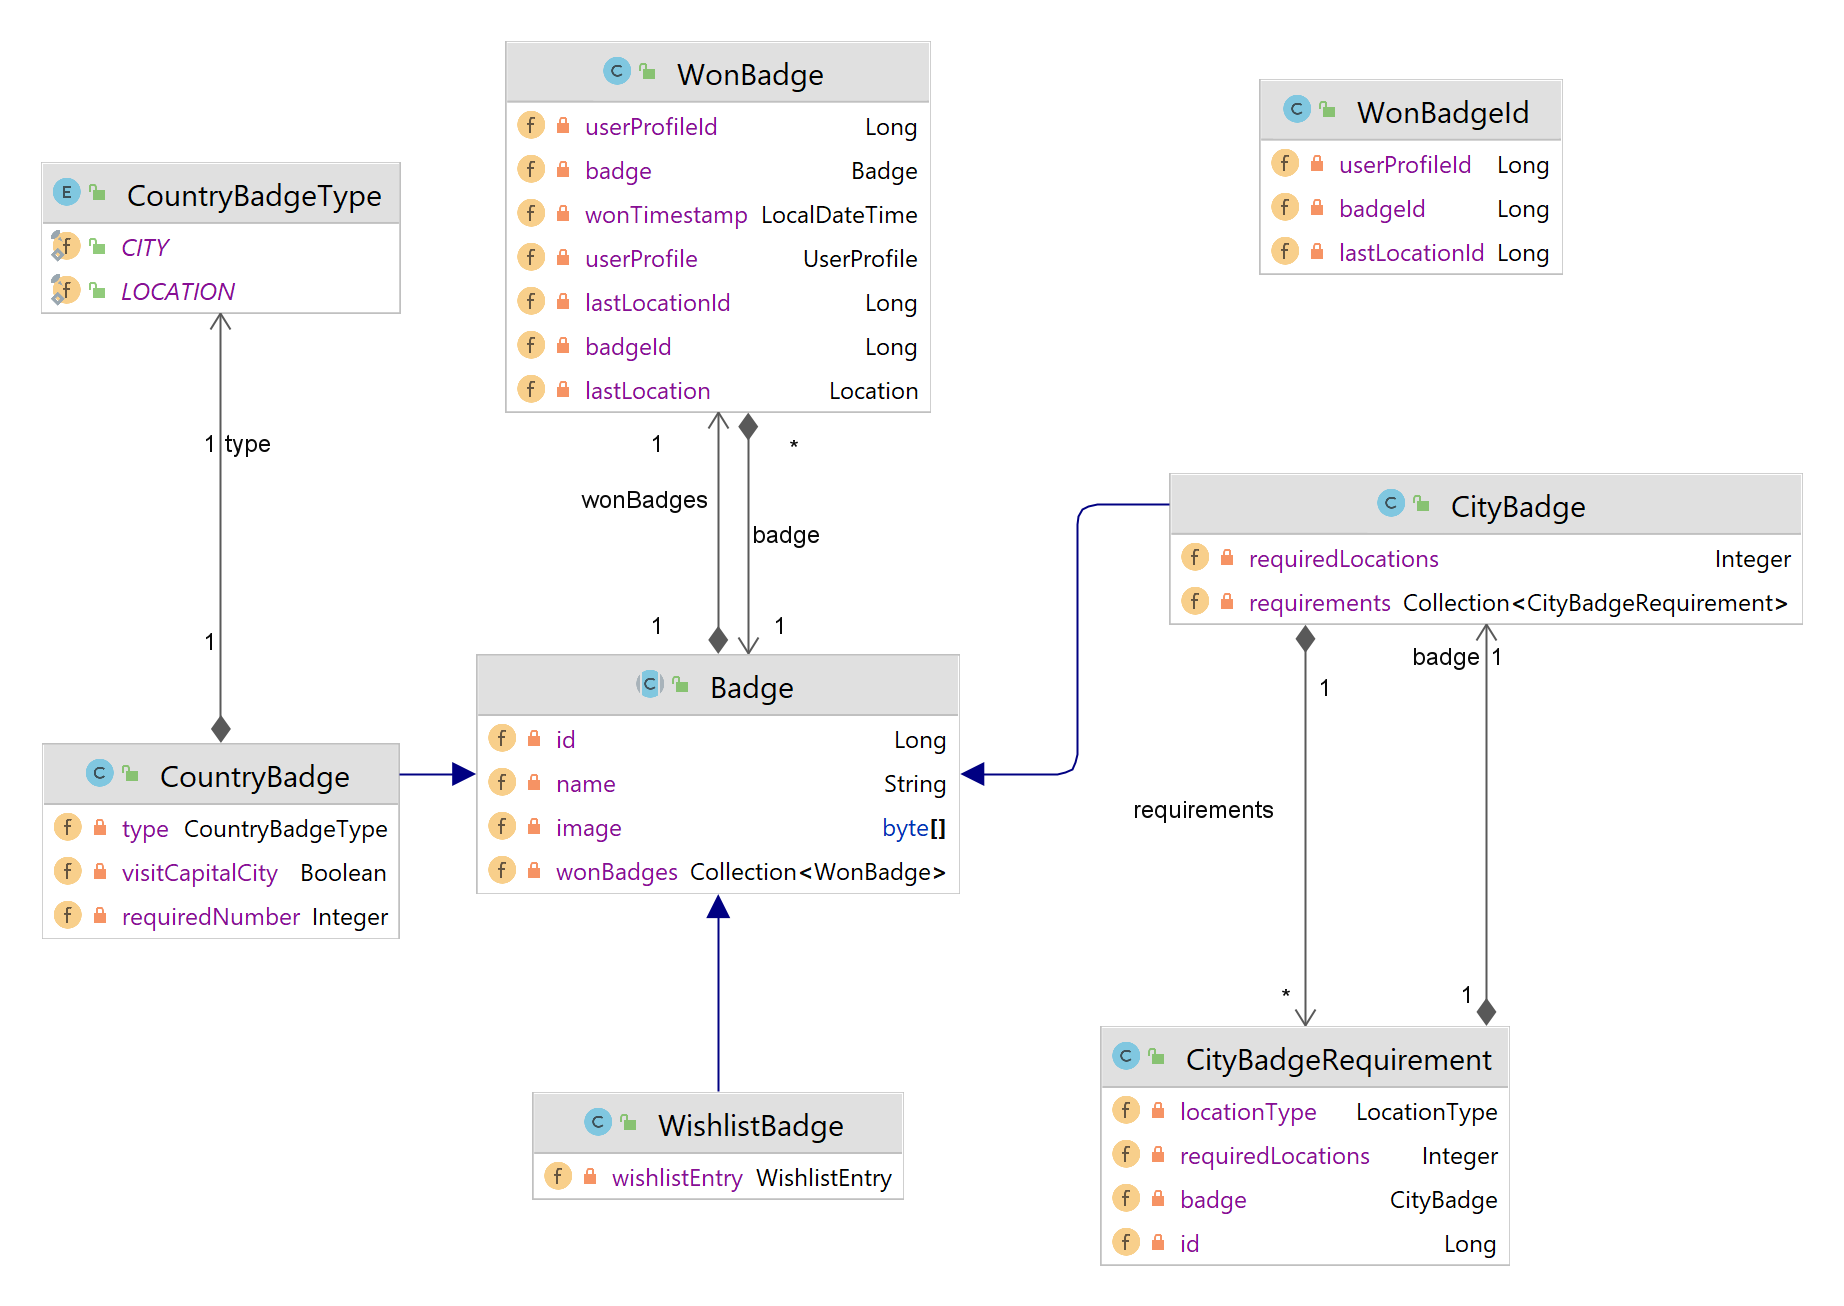
\includegraphics[scale=0.2]{slike/class/class_model_badge.png}
        		\centering
        		\caption{Dijagram razreda - modeli bedževa}
        	\end{figure}
         
                \begin{figure}[H]
        			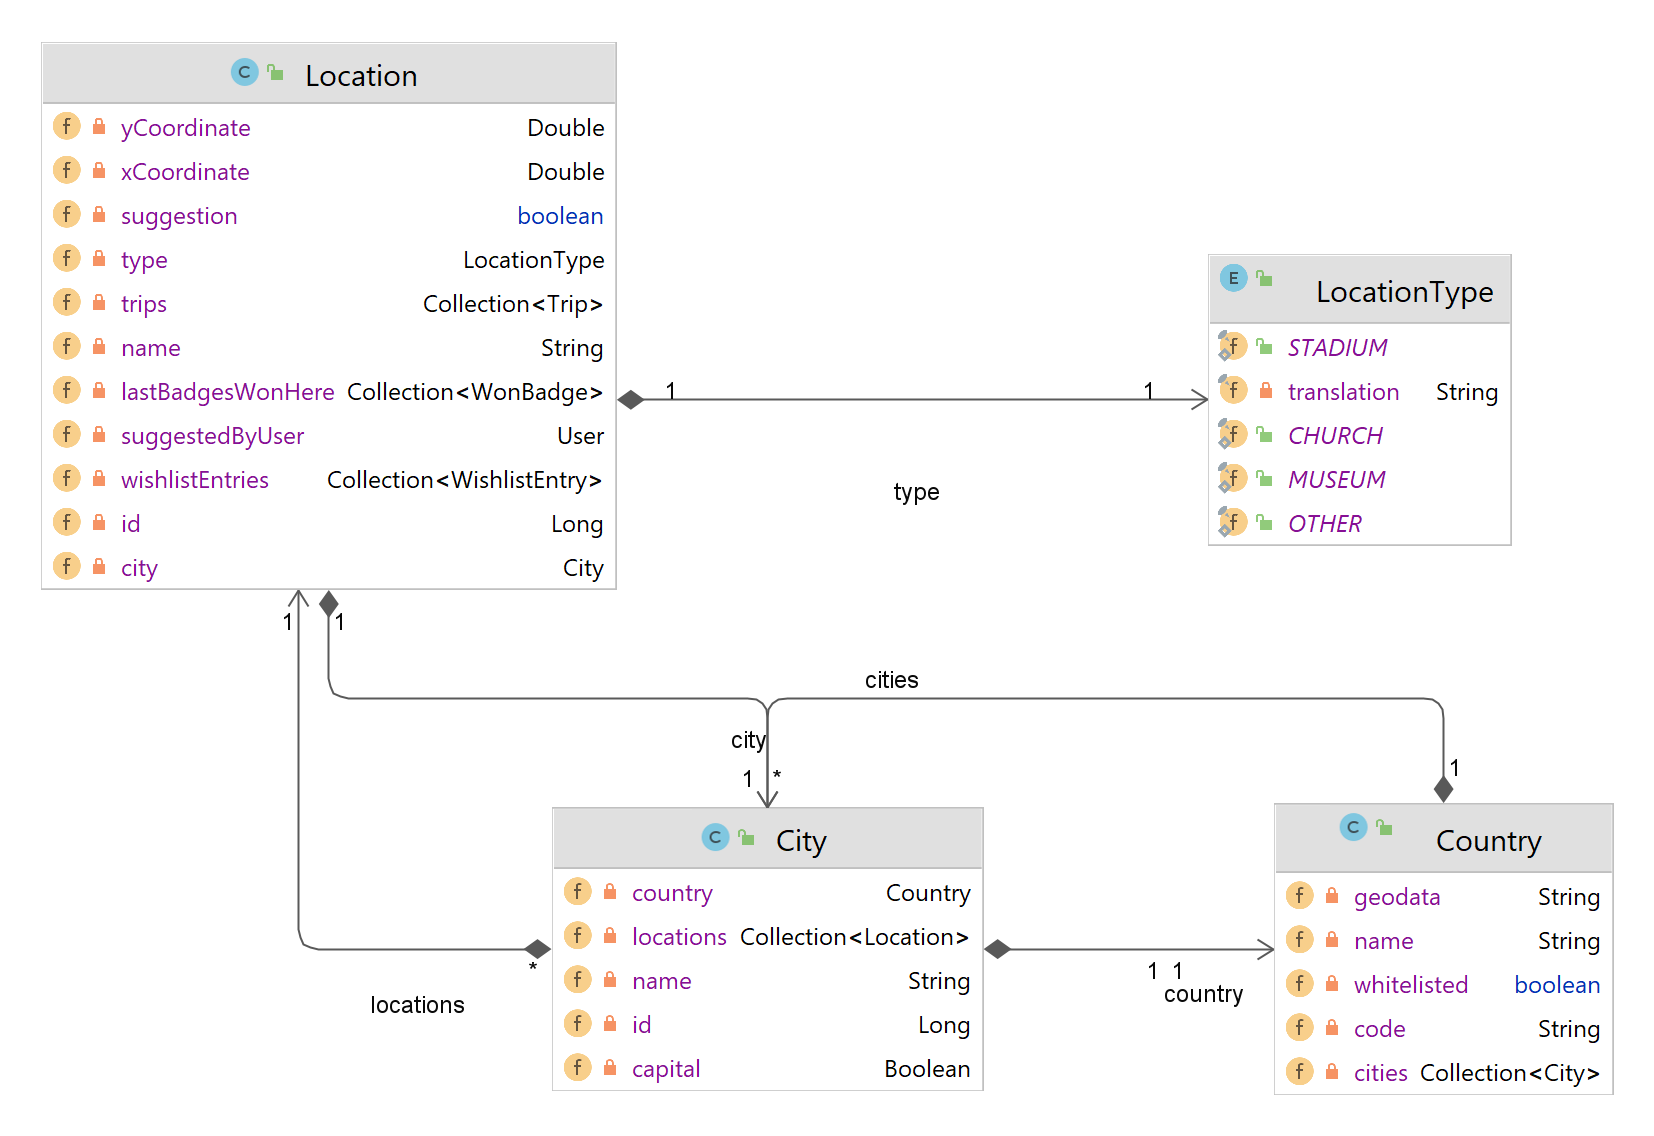
\includegraphics[scale=0.2]{slike/class/class_model_location.png}
        		\centering
        		\caption{Dijagram razreda - modeli lokacija}
        	\end{figure}
         
                \begin{figure}[H]
        			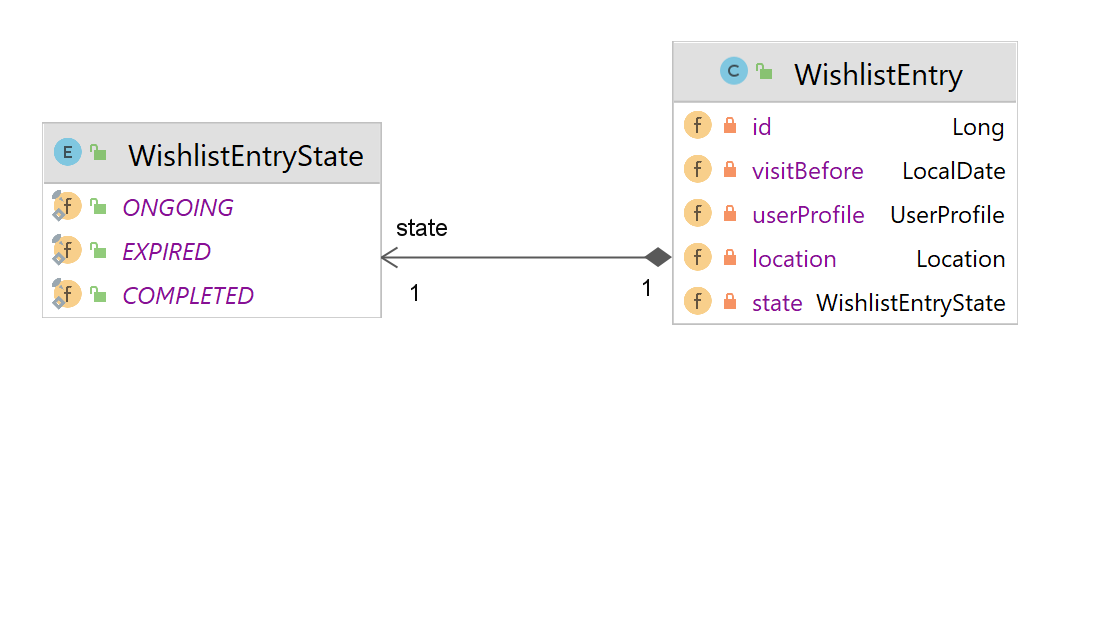
\includegraphics[scale=0.2]{slike/class/class_model_wishlist.png}
        		\centering
        		\caption{Dijagram razreda - modeli \textit{wishlist}-a}
        	\end{figure}

                 Na dijagramima razreda modela prikazani su razredi koji reprezentiraju sve relacije koje predstavljaju neki entitet u bazi podataka, sve vezne relacije koje sadrže dodatne atribute, kompozitne ključeve te enumeracije.
                \\
                \\
                Razredi modela za svako svoje svojstvo imaju metodu \textit{get} i \textit{set} te konstruktore.
                \eject


                \begin{figure}[H]
        			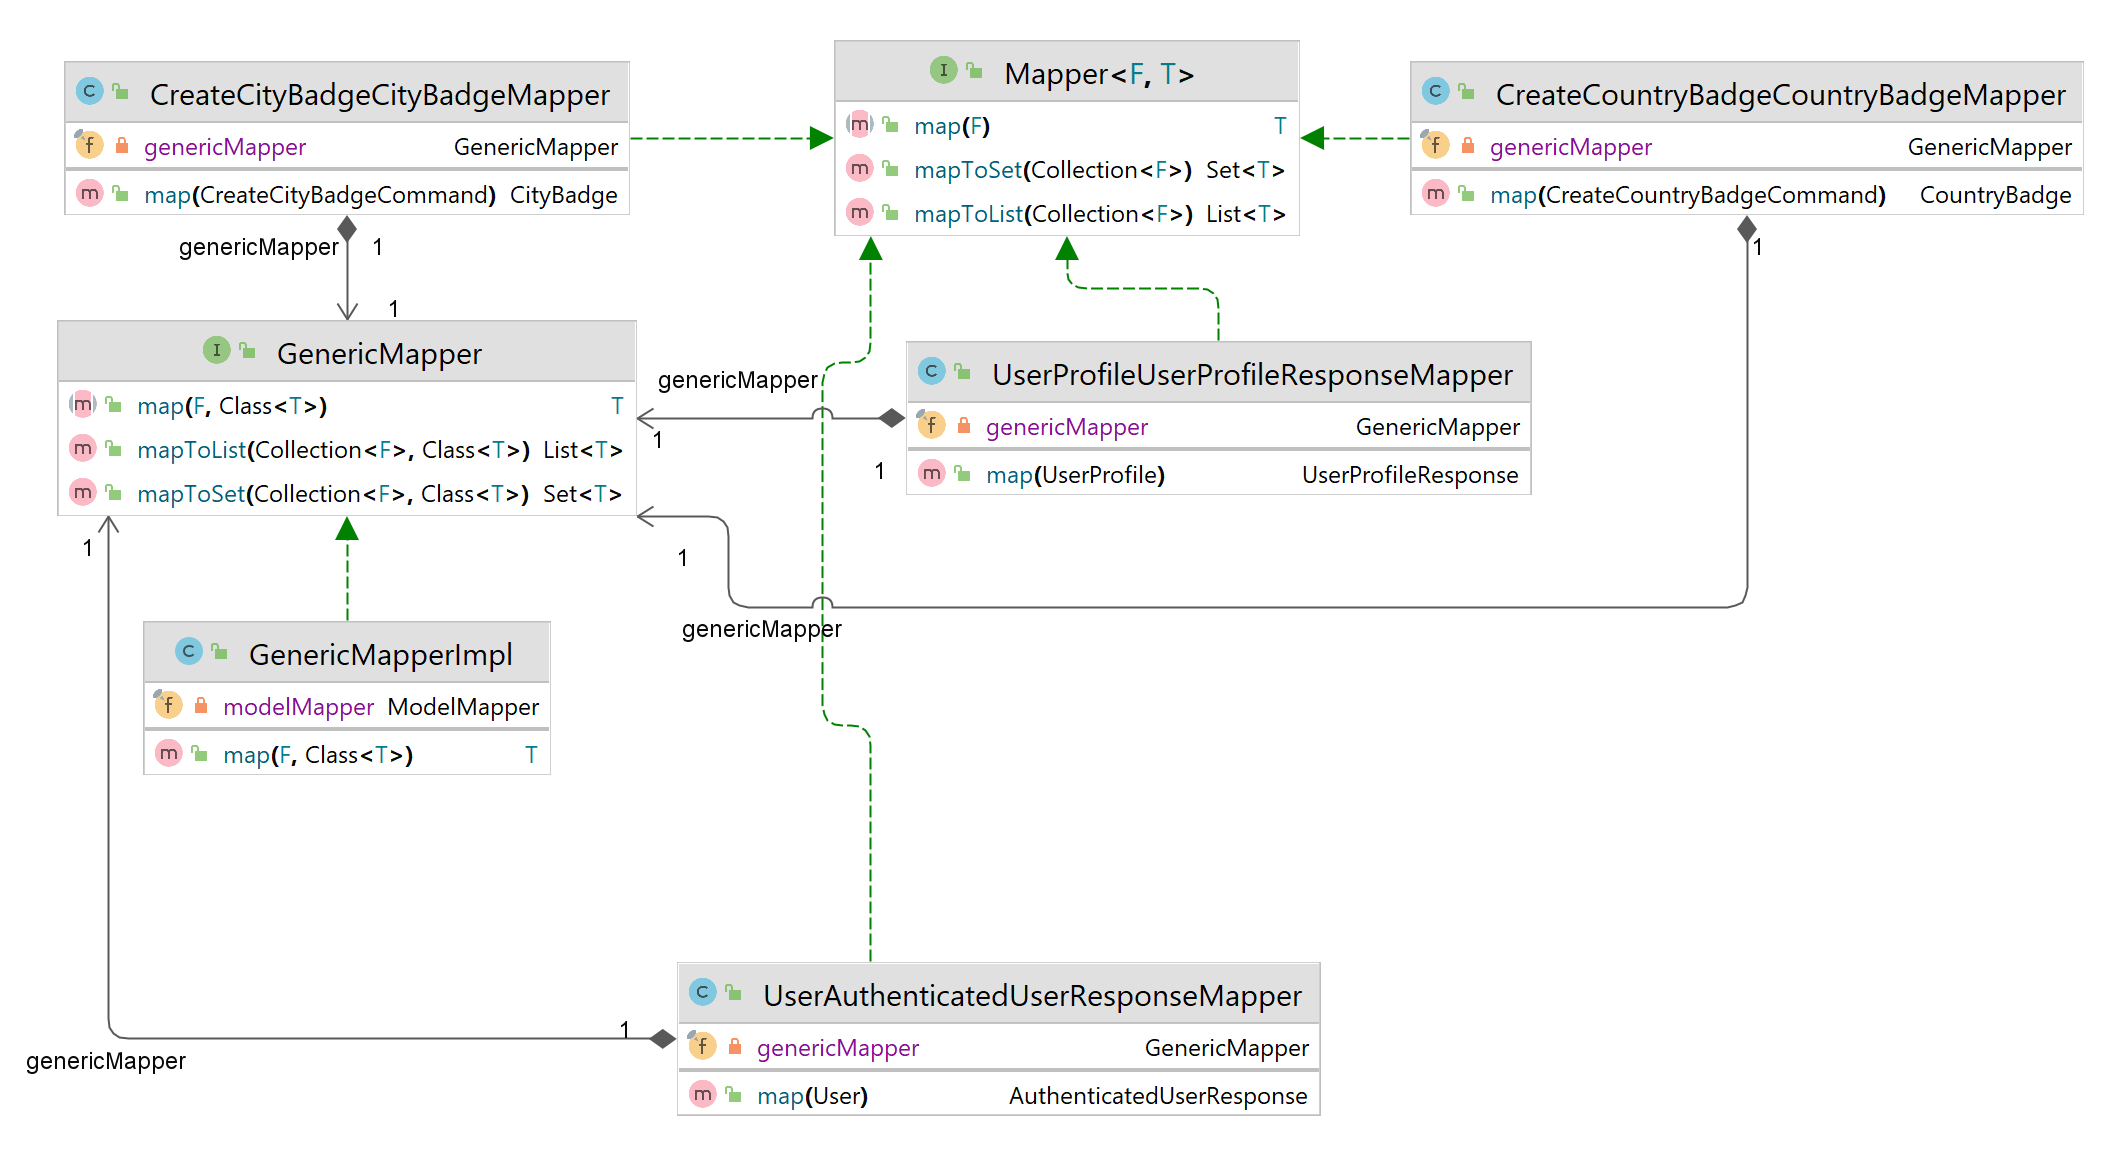
\includegraphics[scale=0.2]{slike/class/class_mapper.png}
        		\centering
        		\caption{Dijagram razreda - \textit{Mapper}}
        	\end{figure}
        

                \begin{figure}[H]
        			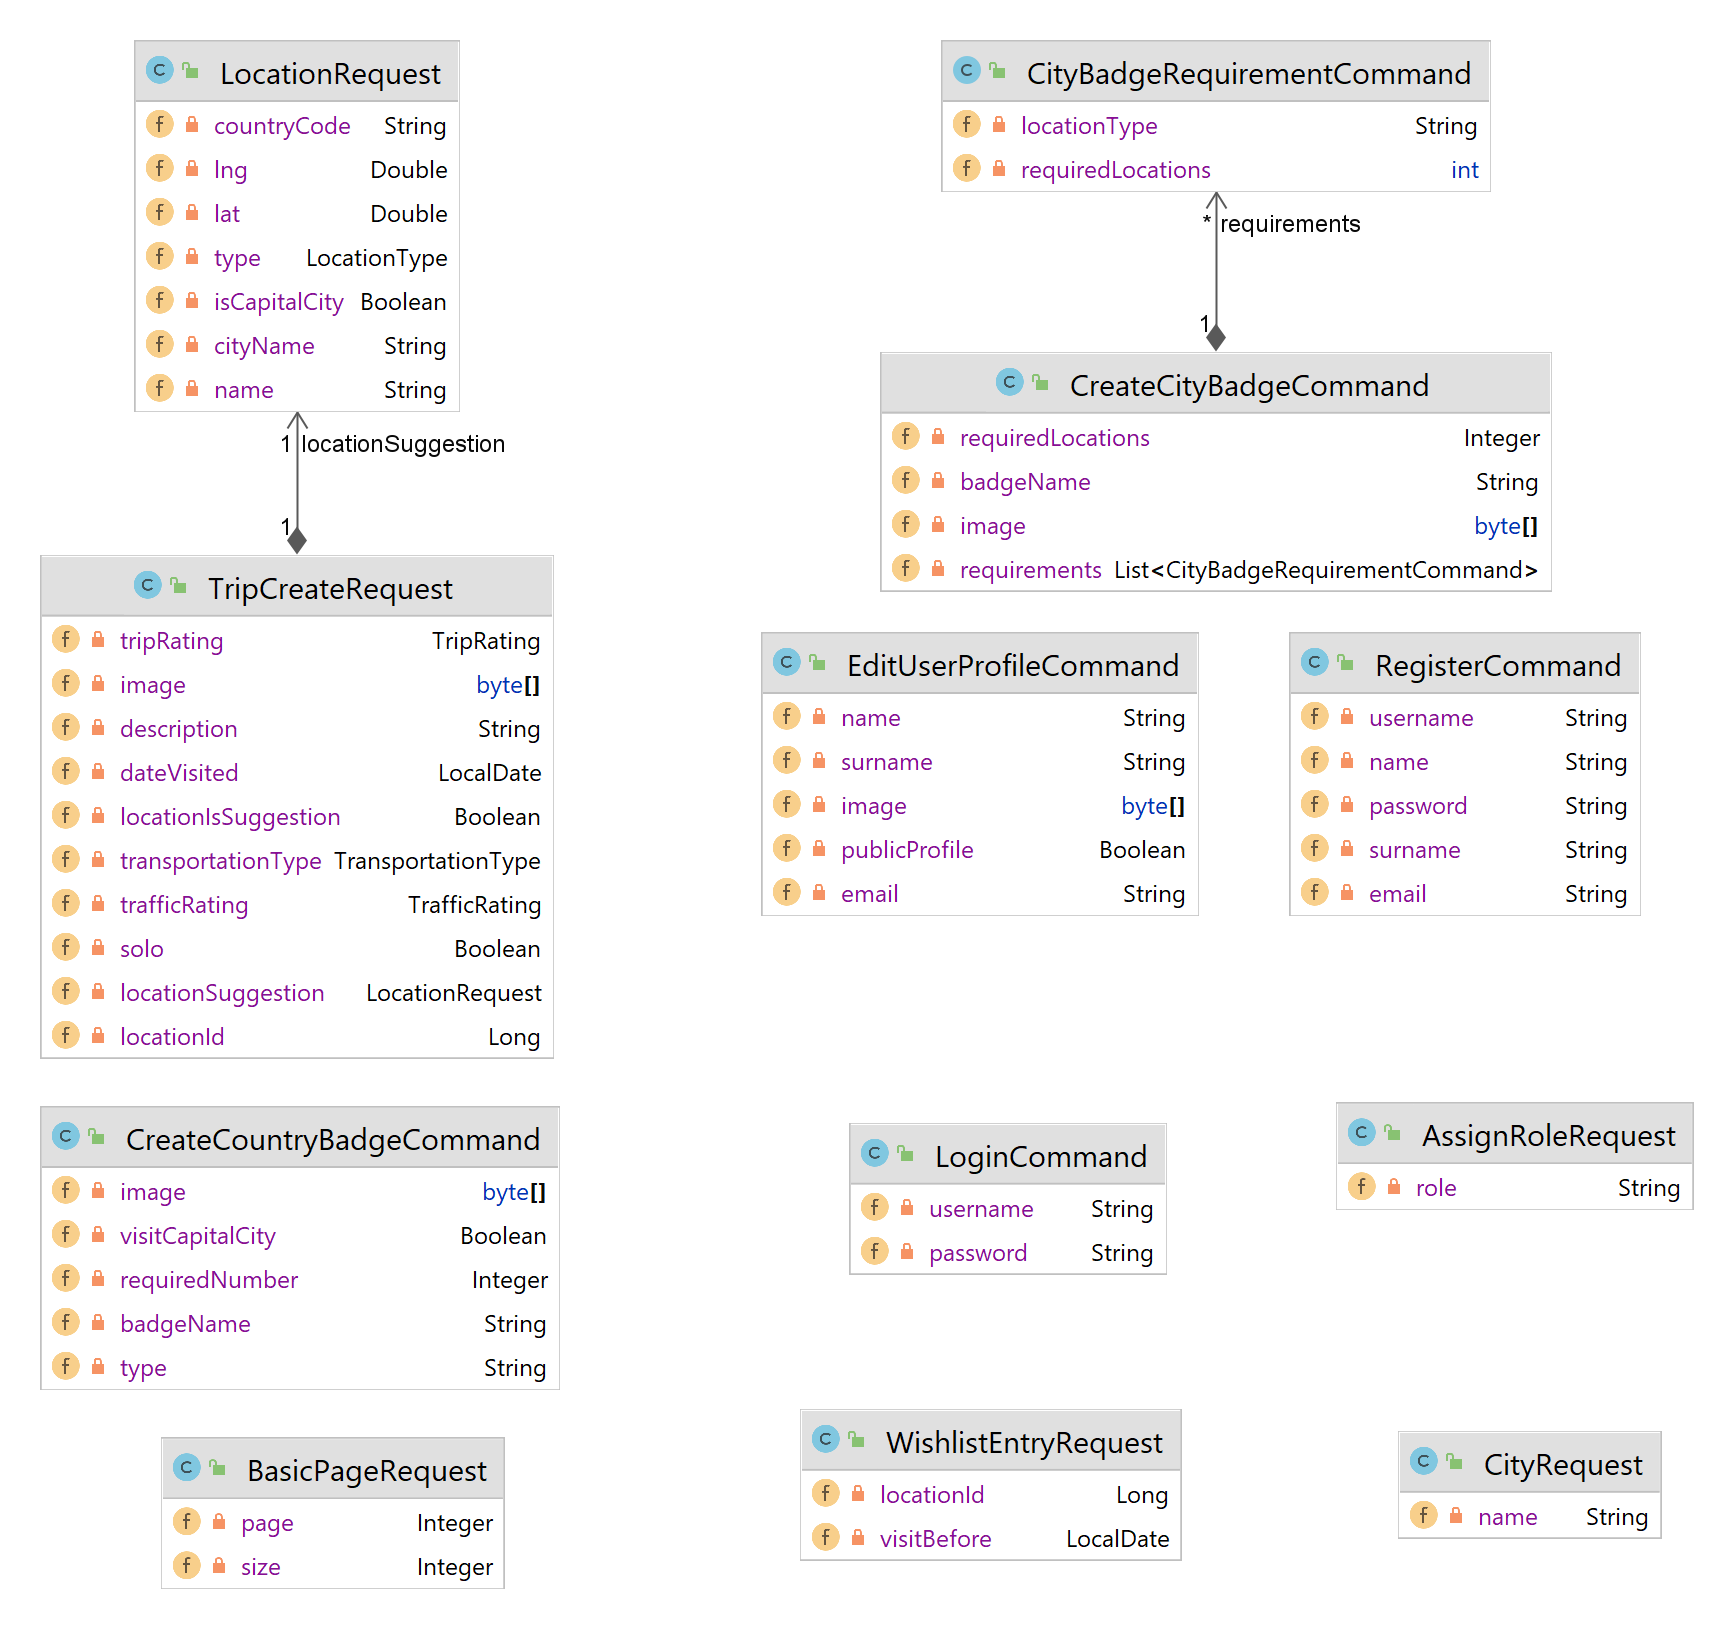
\includegraphics[scale=0.2]{slike/class/class_request.png}
        		\centering
        		\caption{Dijagram razreda - \textit{Request}}
        	\end{figure}

                \begin{figure}[H]
        			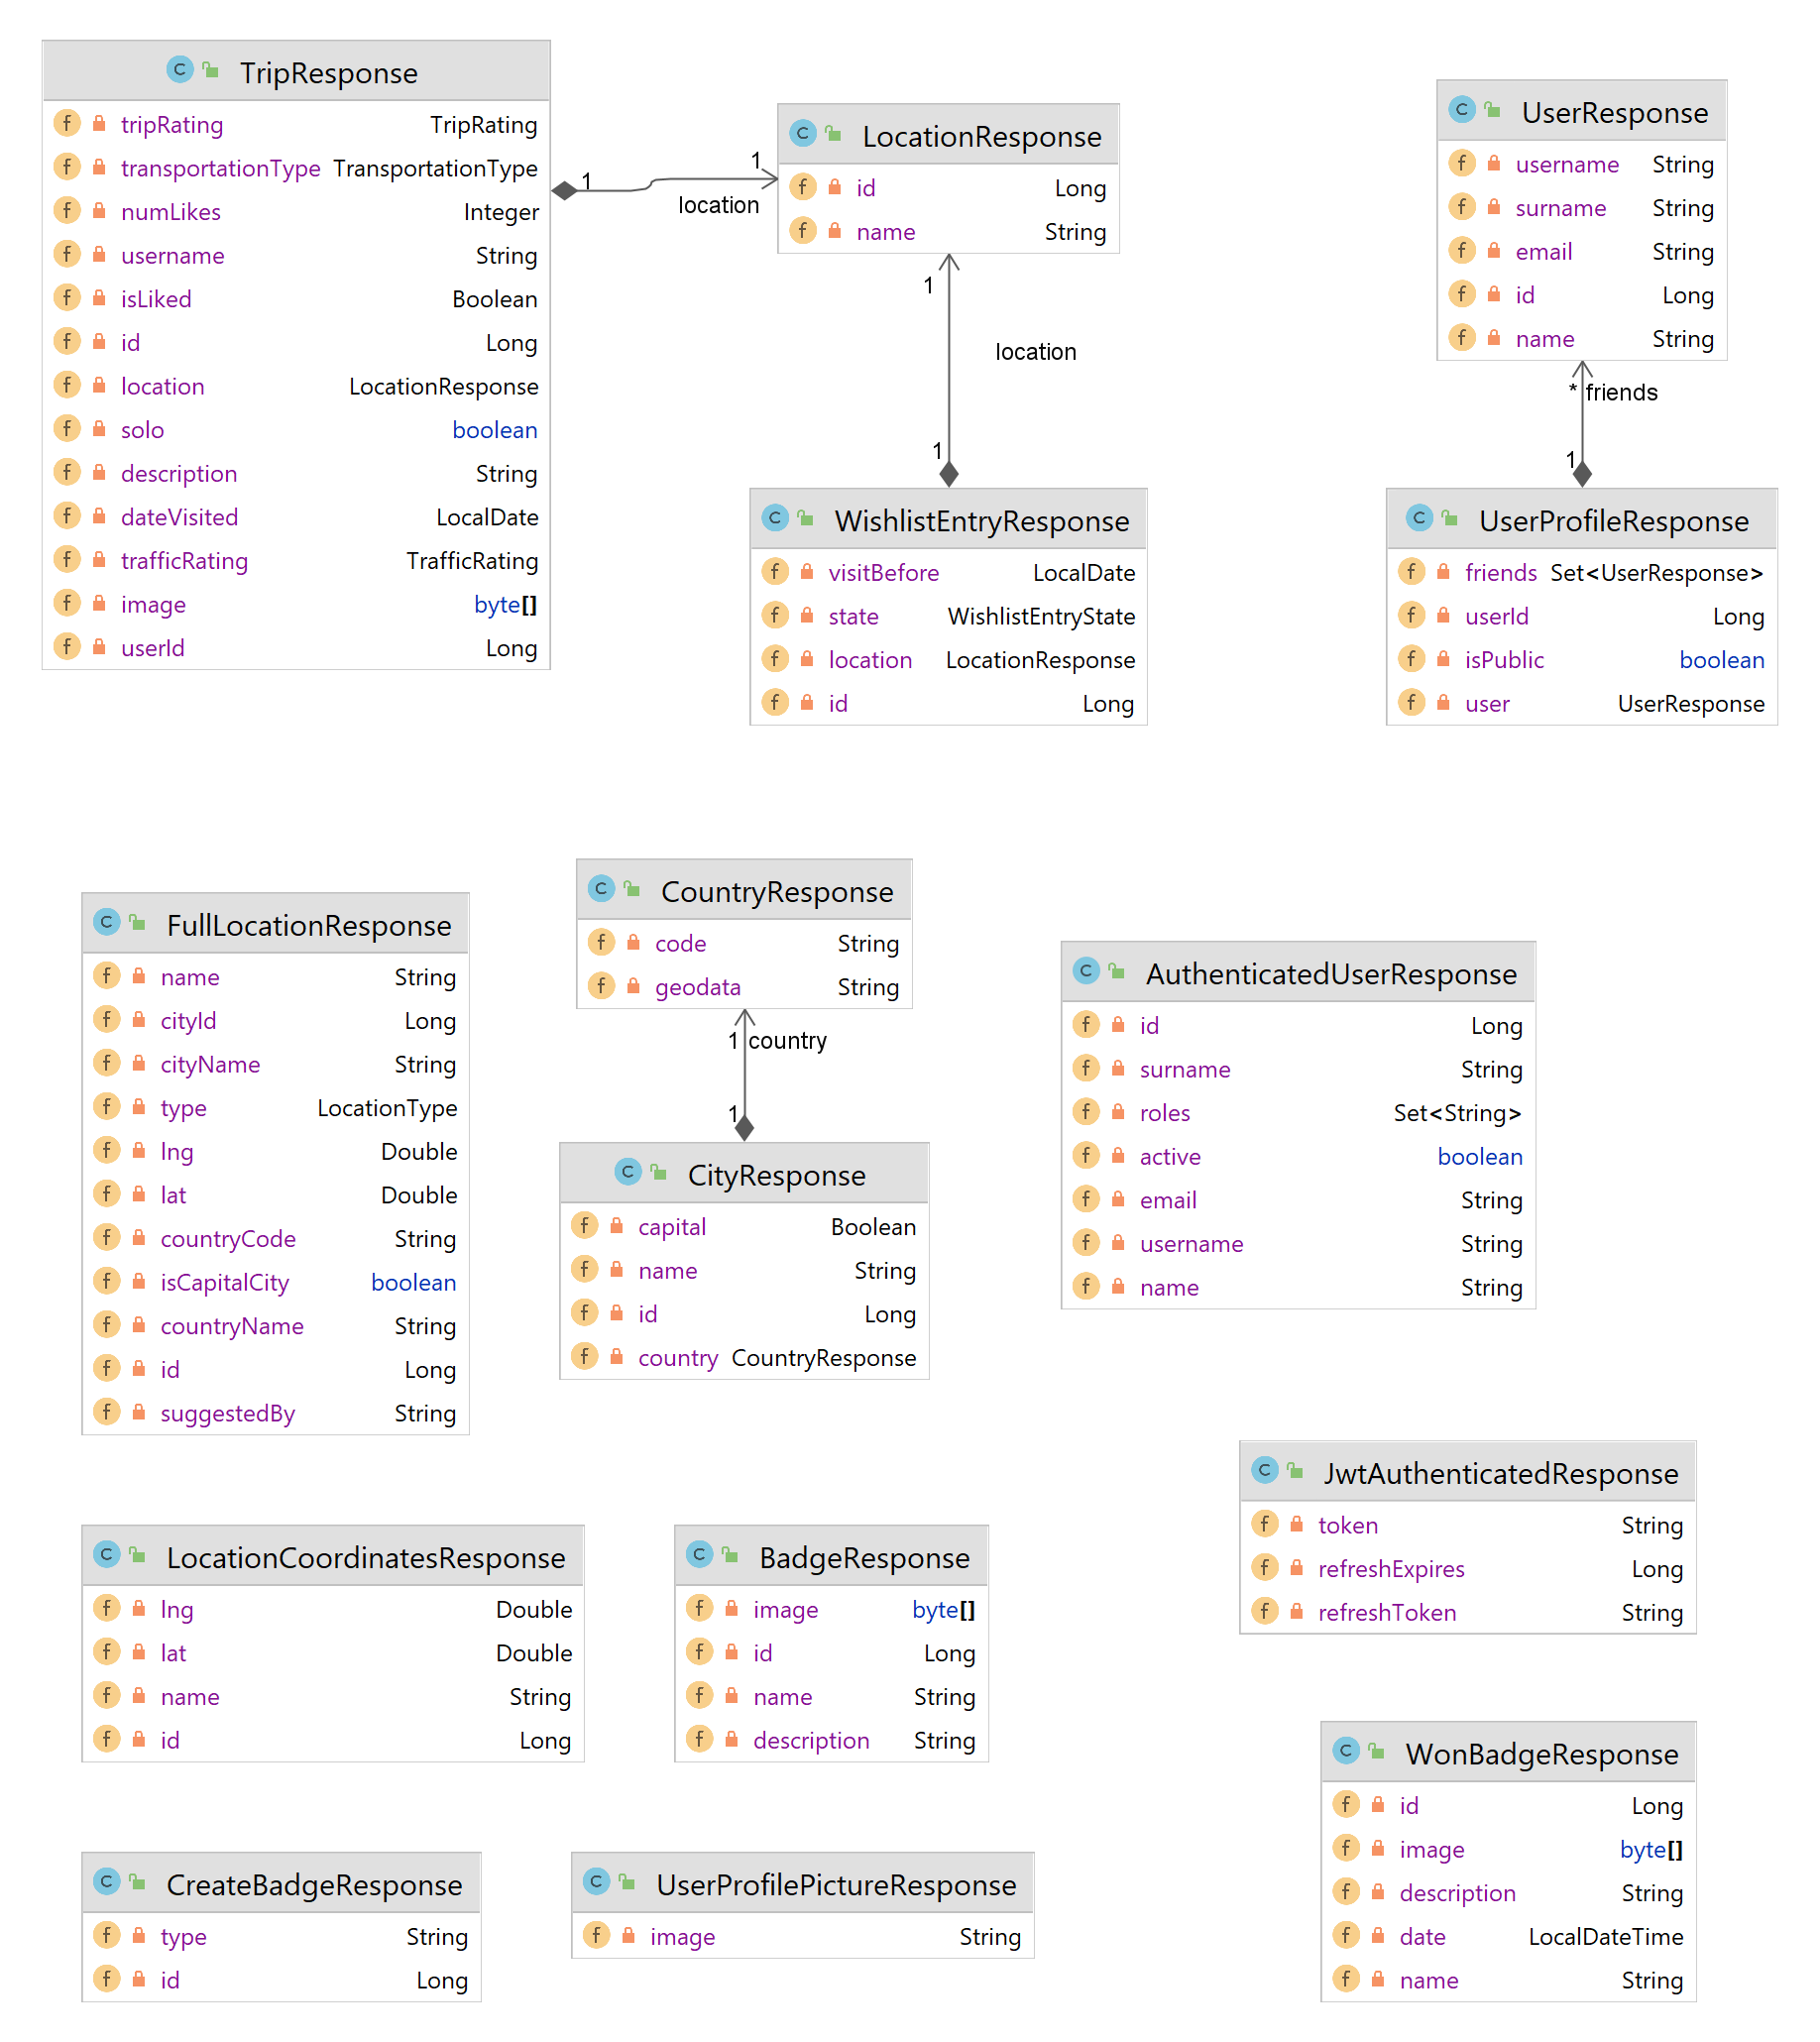
\includegraphics[scale=0.2]{slike/class/class_response.png}
        		\centering
        		\caption{Dijagram razreda - \textit{Response}}
        	\end{figure}
         \eject

                \begin{figure}[H]
        			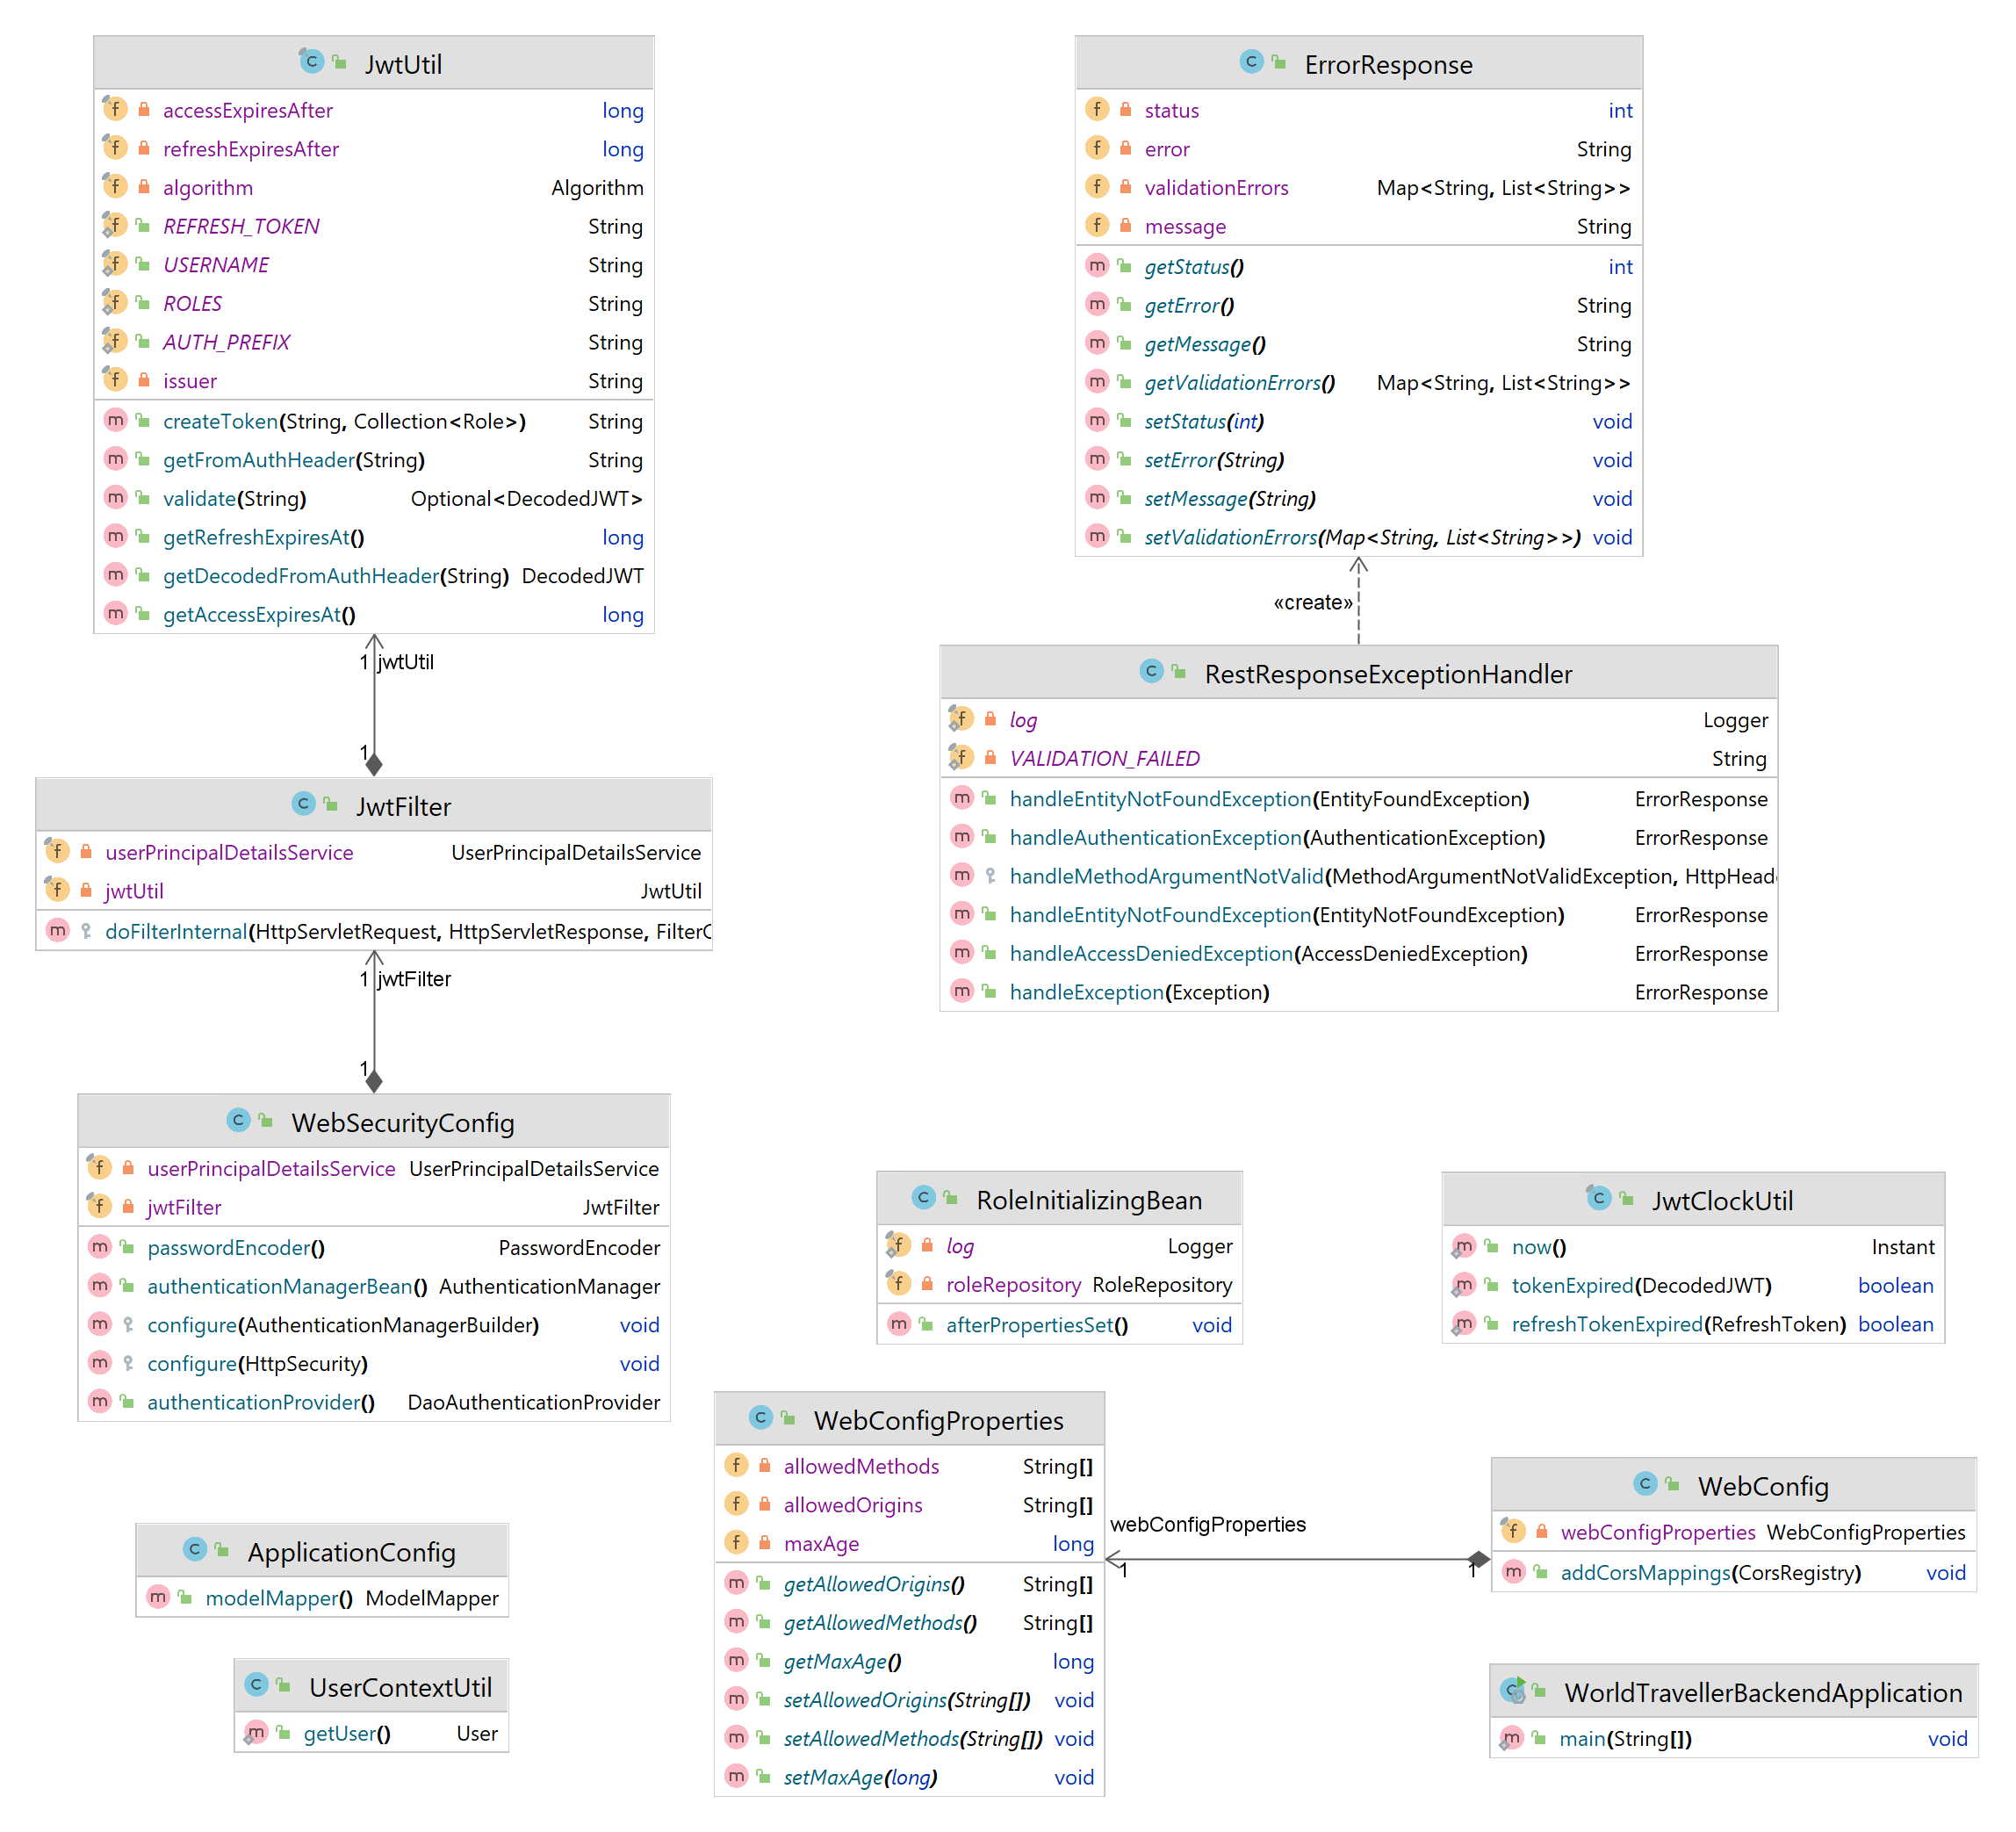
\includegraphics[scale=0.18]{slike/class/class_util_config.png}
        		\centering
        		\caption{Dijagram razreda - konfiguracijski i pomoćni razredi}
        	\end{figure}

			Na dijagramima prikazani su razredi koji se koriste za pokretanje Spring Boot-a, konfiguraciju autorizacije/autentifikacije i filtera, \textit{Exception} i \textit{util} razredi, generički \textit{Mapper} i njegove implementacije koje služi za pretvaranje razreda entiteta u \textit{DTO} (\textit{Request} i \textit{Response}) razred  te još neki konfiguracijski razredi.
            \eject
            
		\section{Dijagram stanja}


			%\textbf{\textit{dio 2. revizije}}\\

			%\textit{Potrebno je priložiti dijagram stanja i opisati ga. Dovoljan je jedan dijagram stanja koji prikazuje \textbf{značajan dio funkcionalnosti} sustava. Na primjer, stanja korisničkog sučelja i tijek korištenja neke ključne funkcionalnosti jesu značajan dio sustava, a registracija i prijava nisu. }
            
            Dijagram stanja prikazuje određenu funkcionalnost aplikacije pomoću automata. Dolje je prikazan dijagram stanja za regularnog korisnika, korisniku se prijavom prvo pokazuje naslovnica odakle može pristupit ostalim dijelovima aplikacije. S obzirom na način kako je implementirano sva "glavna" stanja su međusobno povezana odnosno čine potpuno povezanu mrežu, to su uz "Naslovnica", "Moji bedževi", "Moj profil", "Društvo", "Pretraživanje", "Lista želja" i "Moja putovanja". Iz svih stanja je moguće odjaviti se iz aplikacije. 
            \\
            Pregledavanjem vlastitog profila može se uređivati profil dodatnim klikom.
            Prilikom pretraživanja može se odabrati korisnik i pregledati profil navedenog korisnika.
            Iz stanja "Moja putovanja" moguće je dodati novo putovanje (objavu) ili ukloniti postojeću objavu.
            Na stranici "Lista želja" moguće je dodati novu želju na listu želja ili ukloniti postojeću želju sa liste želja.
            Iz stanja "Društvo" moguće je označiti objave prijatelja oznakom "Sviđa mi se".
            
            
                \begin{figure}[H]
        		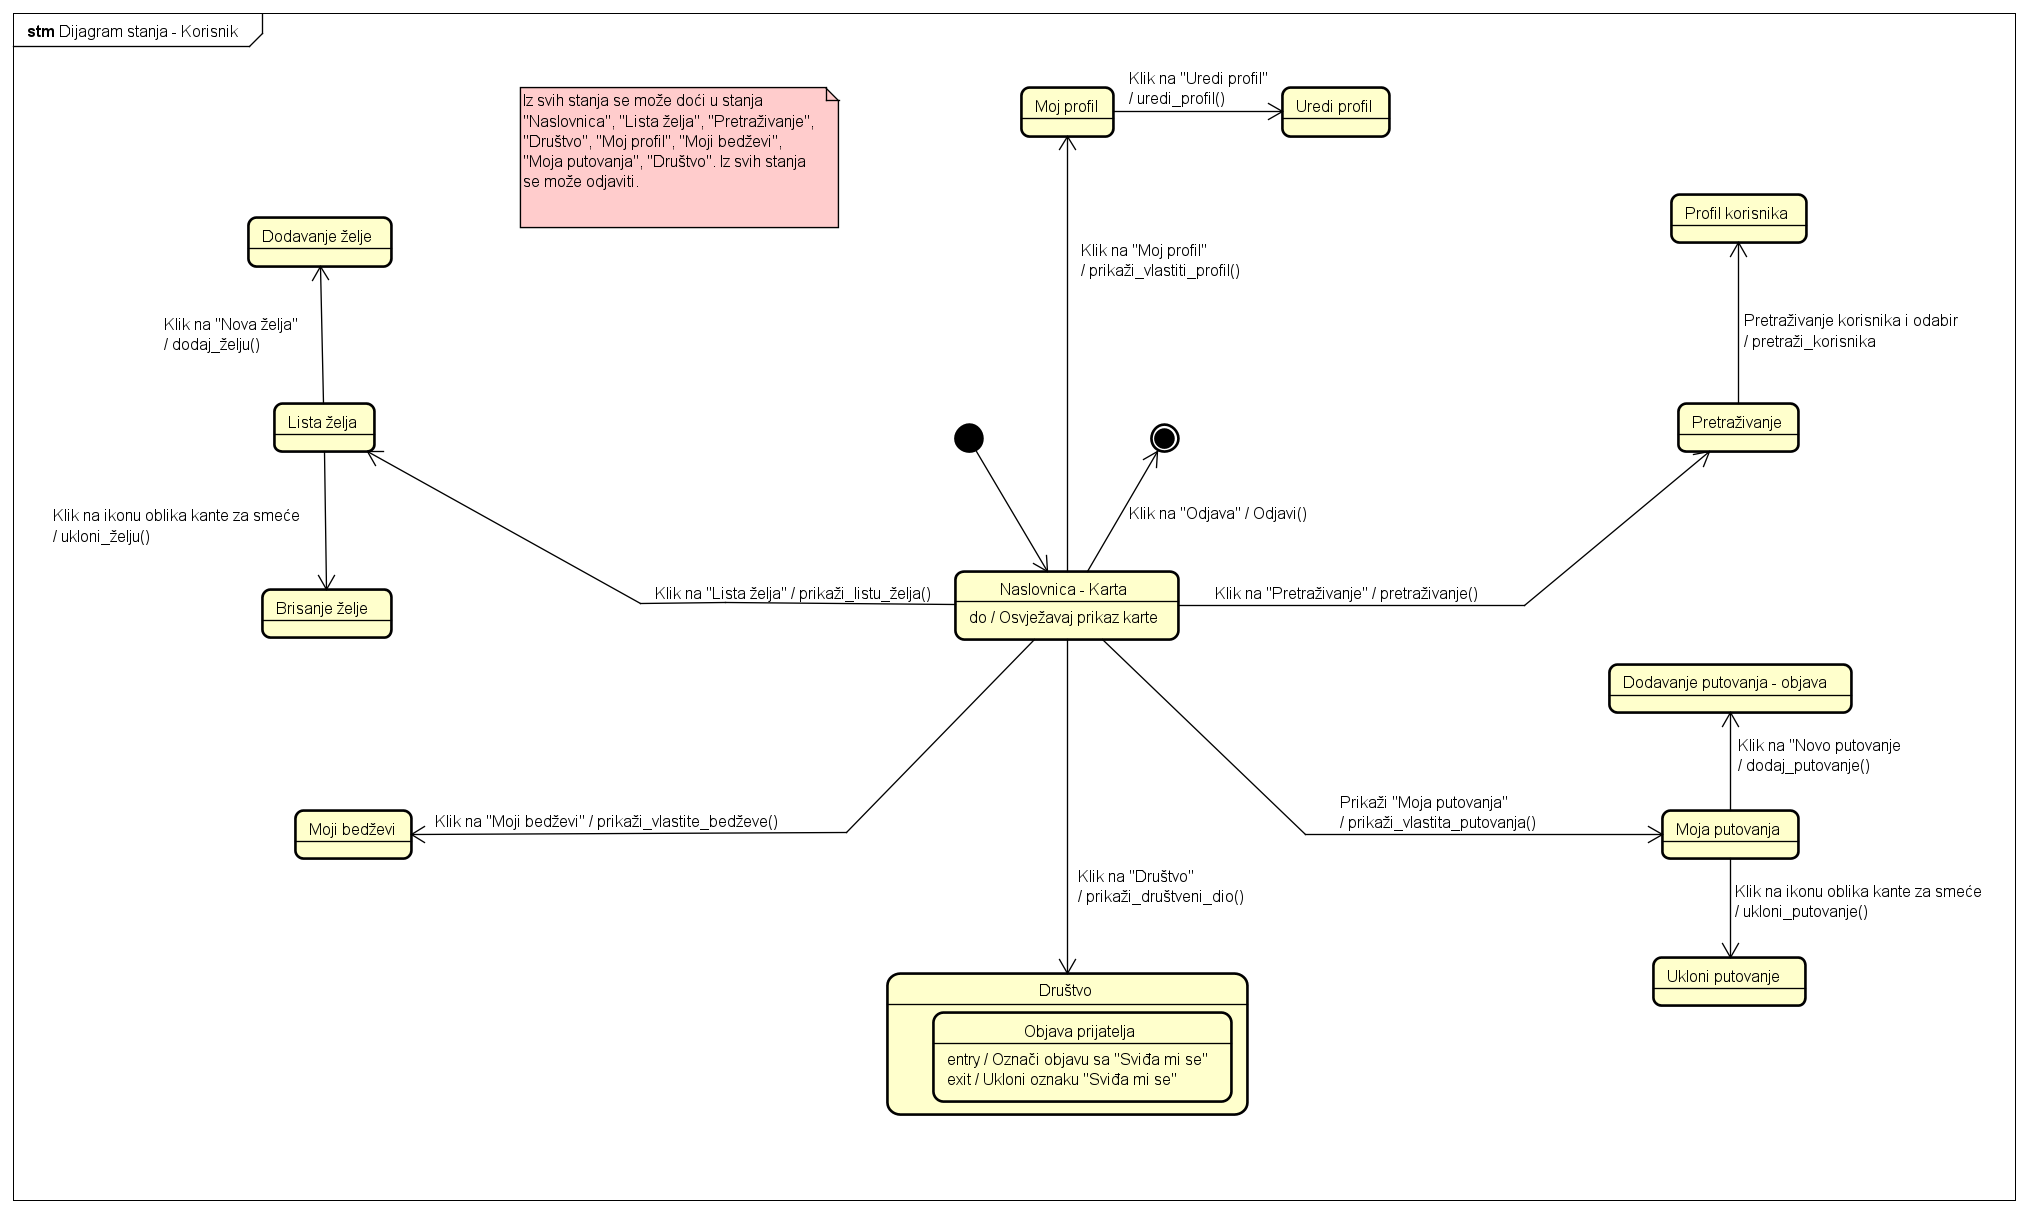
\includegraphics[scale=0.25]{slike/Dijagram stanja - Korisnik.png} %veličina slike u odnosu na originalnu datoteku i pozicija slike
        		  \centering
        		\caption{Dijagram stanja }

        	\end{figure}


			\eject

		\section{Dijagram aktivnosti}

			%\textbf{\textit{dio 2. revizije}}\\

			 %\textit{Potrebno je priložiti dijagram aktivnosti s pripadajućim opisom. Dijagram aktivnosti treba prikazivati značajan dio sustava.}

            Dijagram aktivnosti opisuje tok upravljanja određenog dijela aplikacije. Na dijagramu aktivonsti ispod prikazan je proces objavljivanja putovanja.
            \\
            Korisnik odabire opciju "Nova objava" zatim mu se prikazuje forma za izradu nove objave (putovanja) te mu se prikazuje karta za označavanje mjesta. Nakon provjere označene lokacije i uvjeta bedževa sprema se putovanje (po potrebi lokacija i osvojen bedž) te se korisniku prikazuje stranica s novim putovanjem dodanim.

                \begin{figure}[H]
        		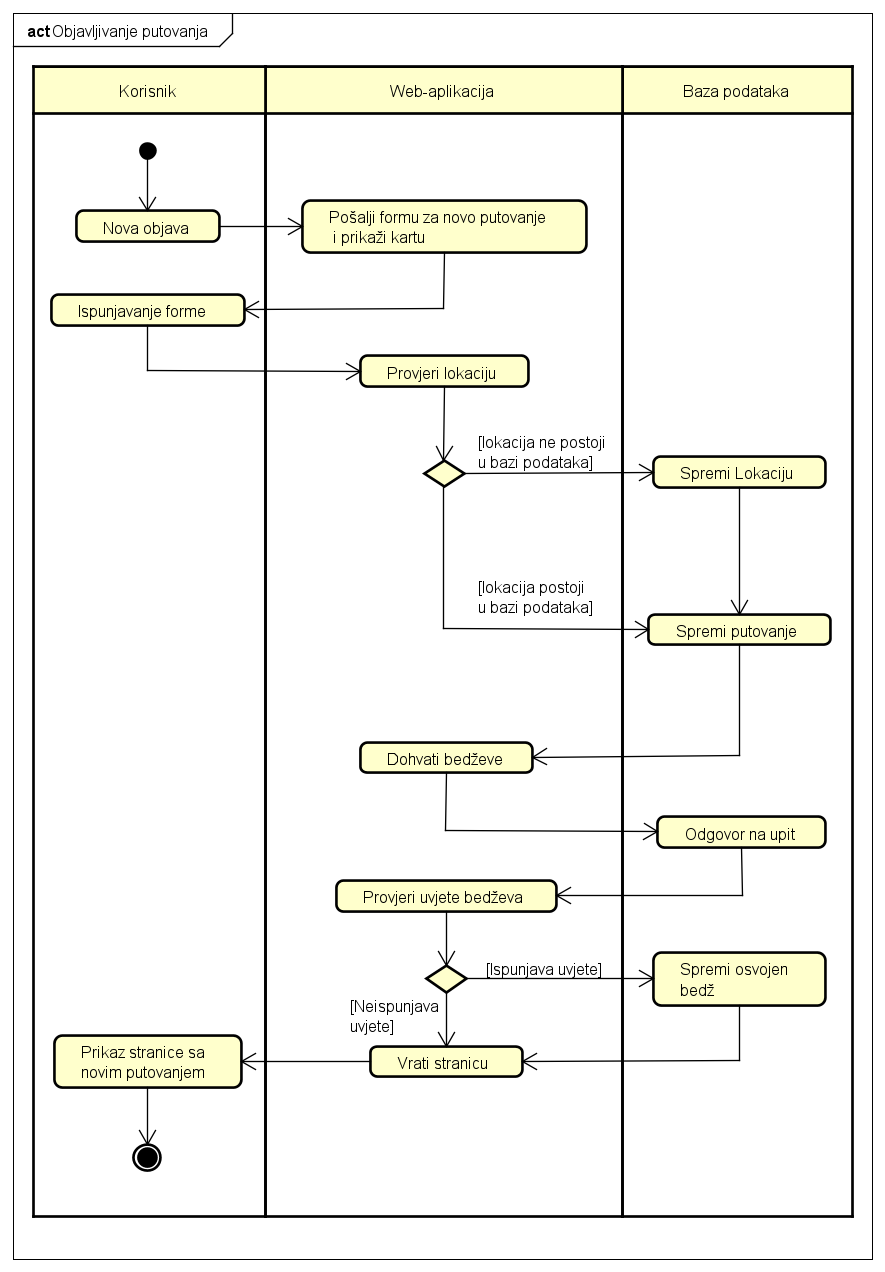
\includegraphics[scale=0.45]{slike/Dijagram aktivnosti - Objavljivanje putovanja.png} %veličina slike u odnosu na originalnu datoteku i pozicija slike
        		  \centering
        		\caption{Dijagram aktivnosti }

        	\end{figure}
         
			\eject
		\section{Dijagram komponenti}

			%\textbf{\textit{dio 2. revizije}}\\

			 %\textit{Potrebno je priložiti dijagram komponenti s pripadajućim opisom. Dijagram komponenti treba prikazivati strukturu cijele aplikacije.}
            

            Dijagram komponenti prikazuje organizaciju i internu strukturu aplikacije. Na dijagramu komponenti ispod prikazana je struktura aplikacije Svjetski putnik.
            Sustavu se pristupa preko dva sučelja, jednim koji komunicira sa dijelom \textit{frontenda} i jednim koji komunicira sa dijelom \textit{backenda} (i baze podataka). Preko sučelja za dohvat CSS, JS i TS datoteka poslužuju se datoteke koje pripadaju \textit{frontend} dijelu, a preko sučelja za dohvat JSON datoteka poslužuju se datoteke koje pripadaju \textit{backend} dijelu.
            \\
            Sve JS/TS datoteke ovise o React \textit{library-u} iz koje dohvaćaju potrebne komponente. REST API poslužuje podatke koji pripadaju \textit{backend} dijelu aplikacije, odnosno pruža JSON podatke. JPA je zadužen za dohvaćanje tablica iz baze podataka.

                \begin{figure}[H]
        		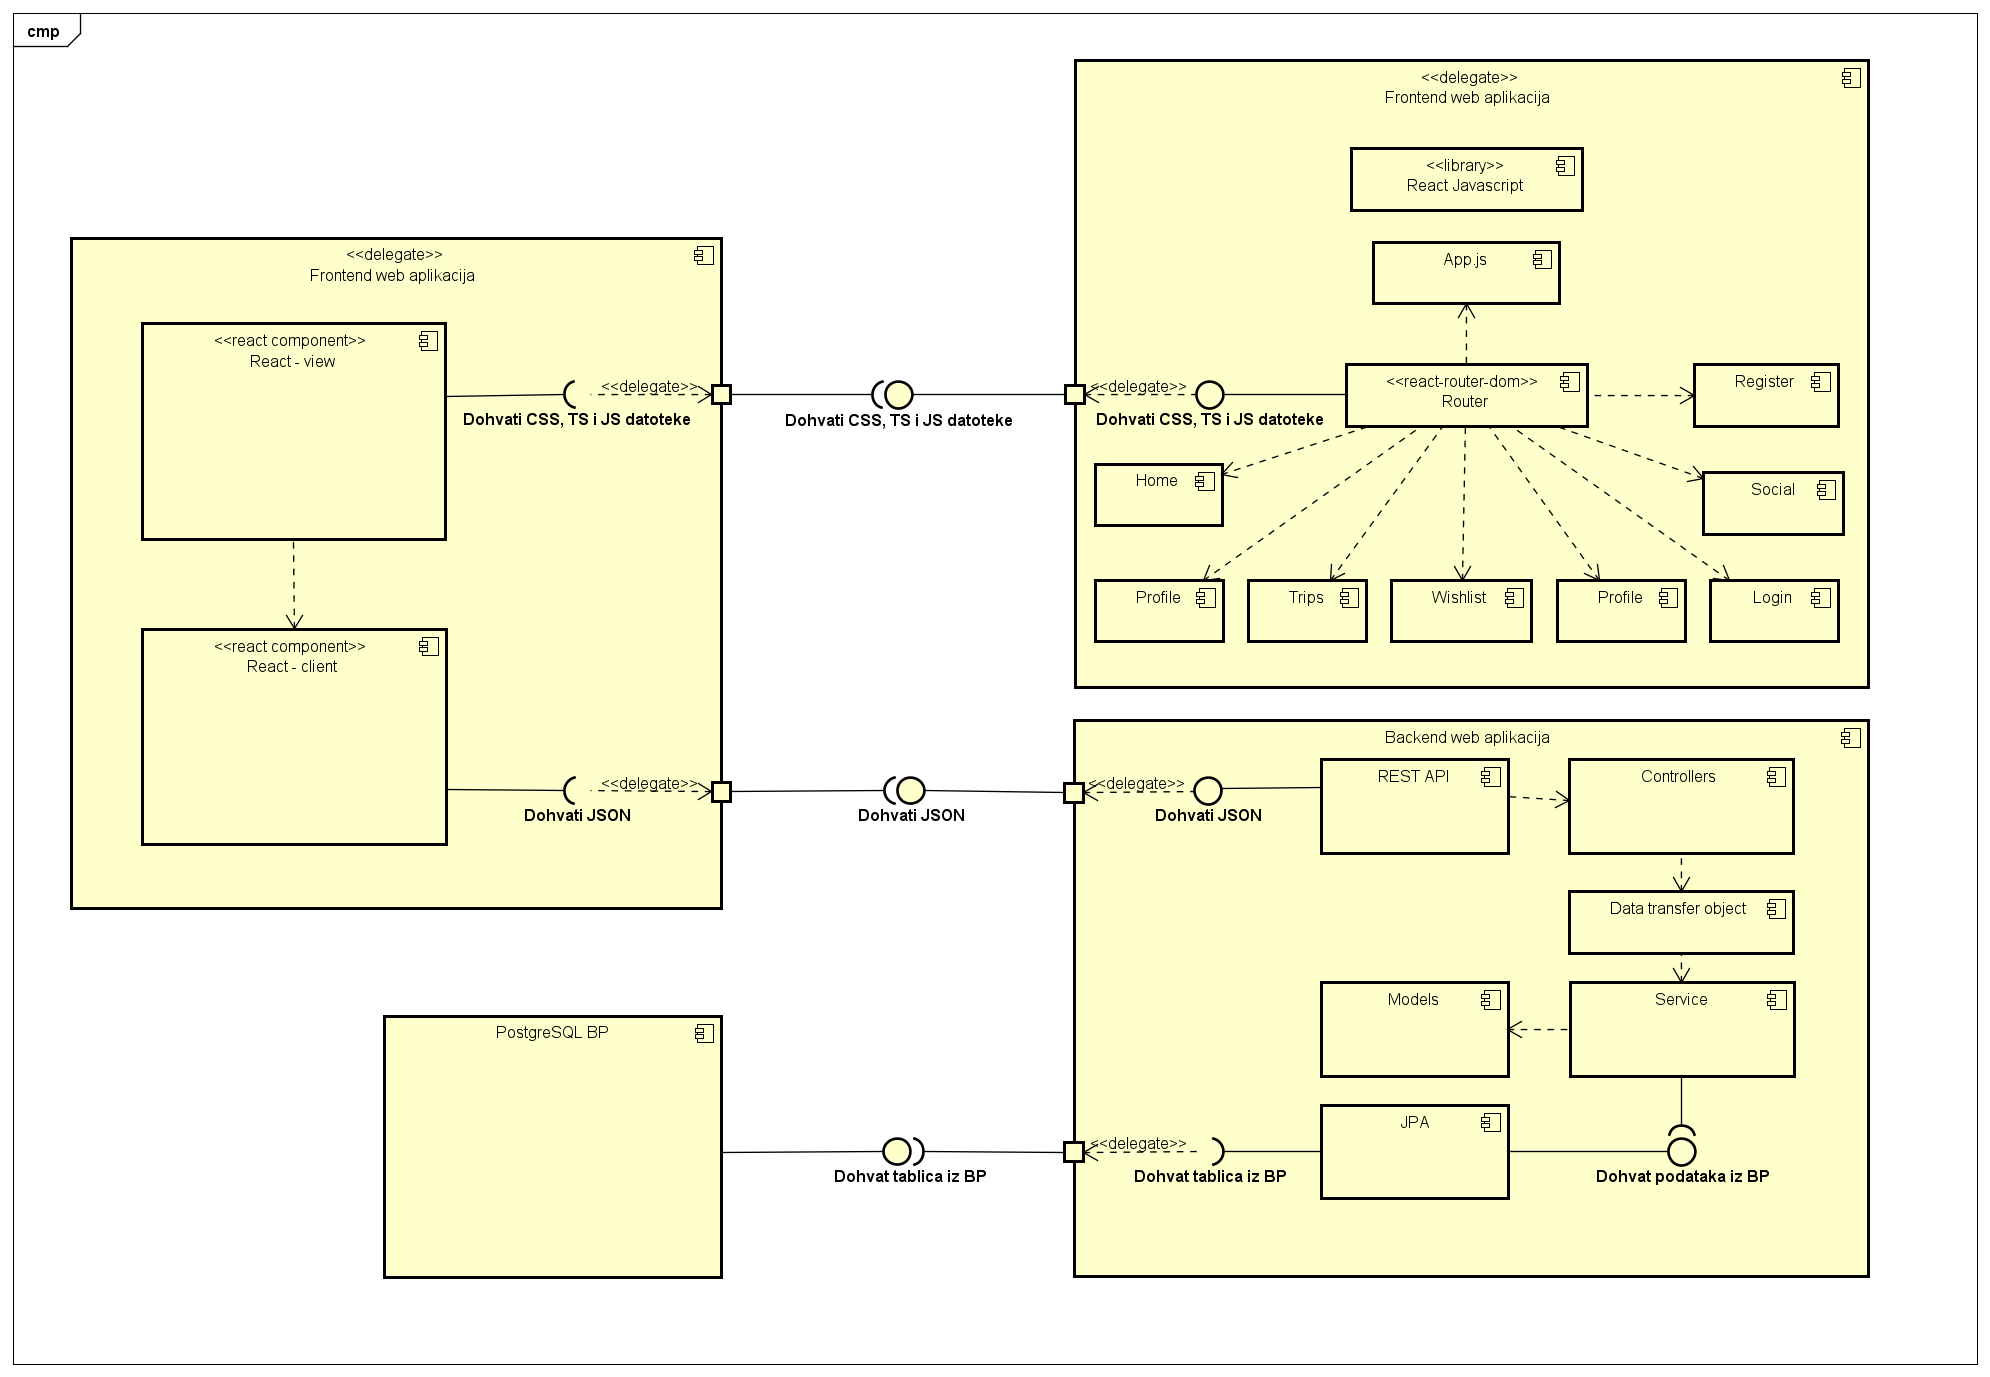
\includegraphics[scale=0.3]{slike/Dijagram komponenti.png} %veličina slike u odnosu na originalnu datoteku i pozicija slike
        		  \centering
        		\caption{Dijagram komponenti}

        	\end{figure}
         \eject